\section{Supporting Simulations with OpenFOAM}

\subsection{Case Setup GUI: \texttt{isofCaseBuilder}}

\subsection{Execution Monitor GUI: \texttt{isofExecutionManager}}

\subsection{Tabular Output Data Plot: \texttt{isofPlotTabular}}

\subsection{Common Tasks in the Context of OpenFOAM Simulations}

\subsubsection{Meshing}



\paragraph{Extraction of Feature Edges from STL Geometries}

Features edges can be extracted automatically from STLs. 
They are usually found by looking at the angle between neighbouring triangular facets.
This methods is usually automatically applied either in snapphyHexMesh itself or within InsightCAE's workflows.
This method works nicely for edges between planar surfaces.
Though it fails e.g. for rounded edges like leading and trailing edges of propellers and foils.
In such cases, it is required to extract feature edges manually and feed them into the meshing process.

Here, it is described how to extract feature curves using the open source software Blender\footnote{\url{https://www.blender.org/}}.
The following steps are required:
\begin{enumerate}
\item Import the geometry into Blender

select in menu \menu{File>Import>STL (*.stl)}

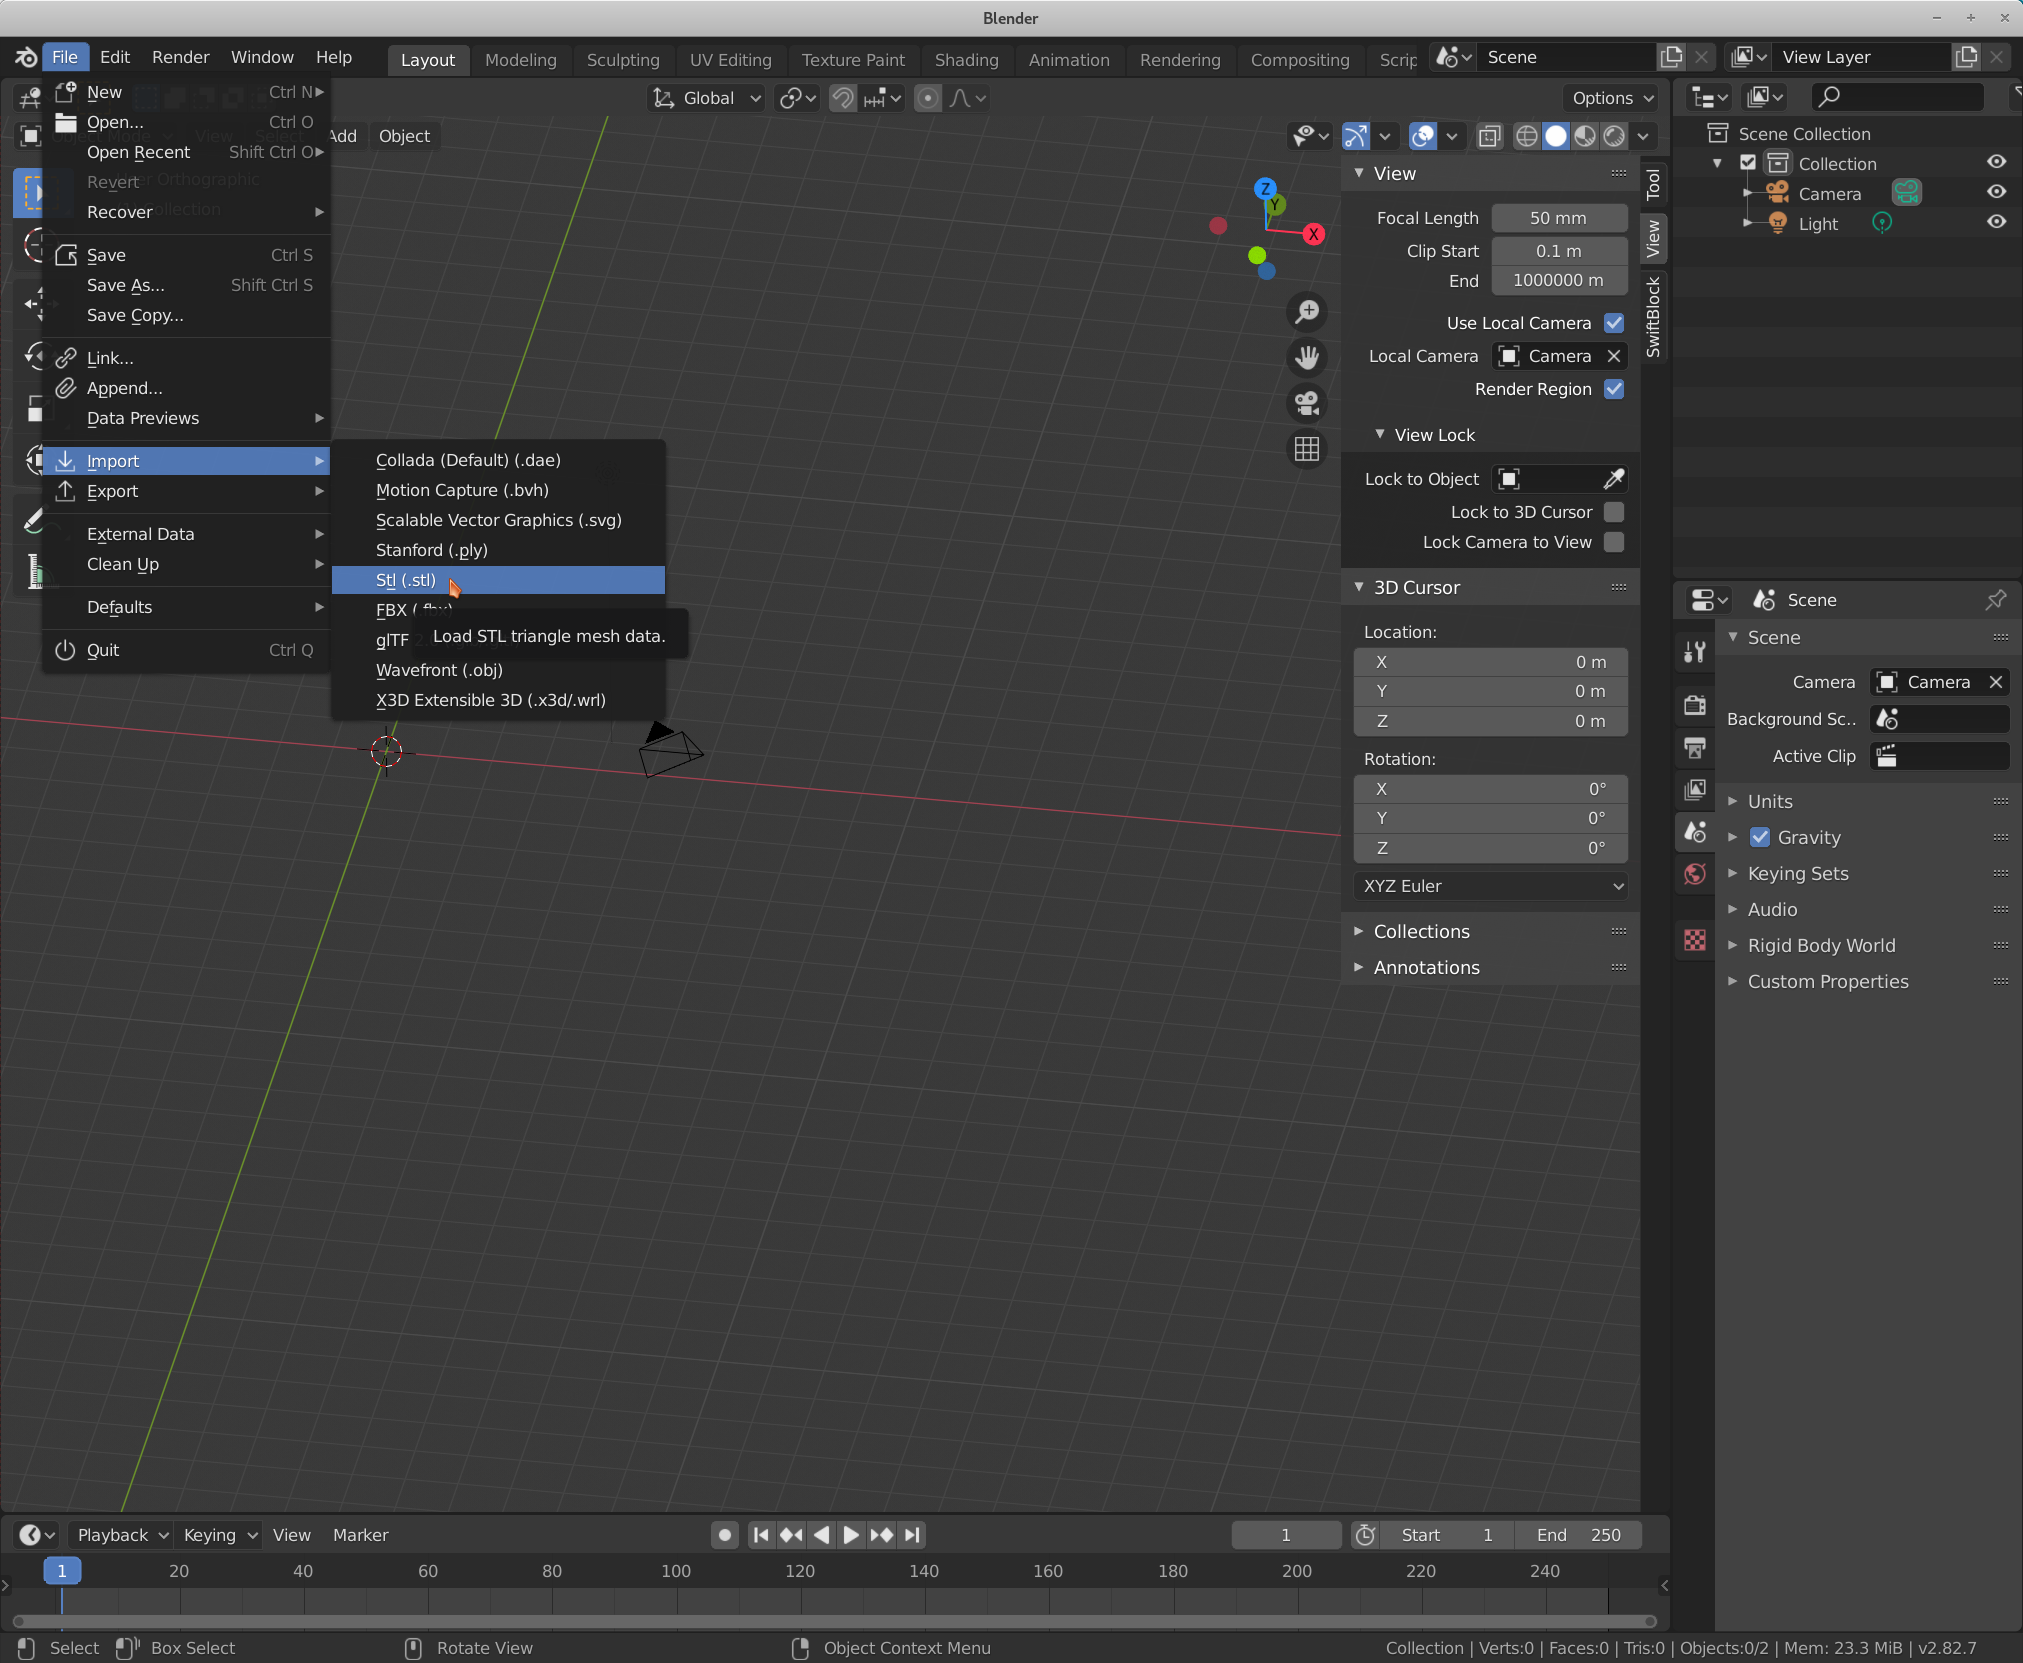
\includegraphics[width=0.75\linewidth]{figs/feature_edges_blender/01_import_stl_1}

\item select the STL file

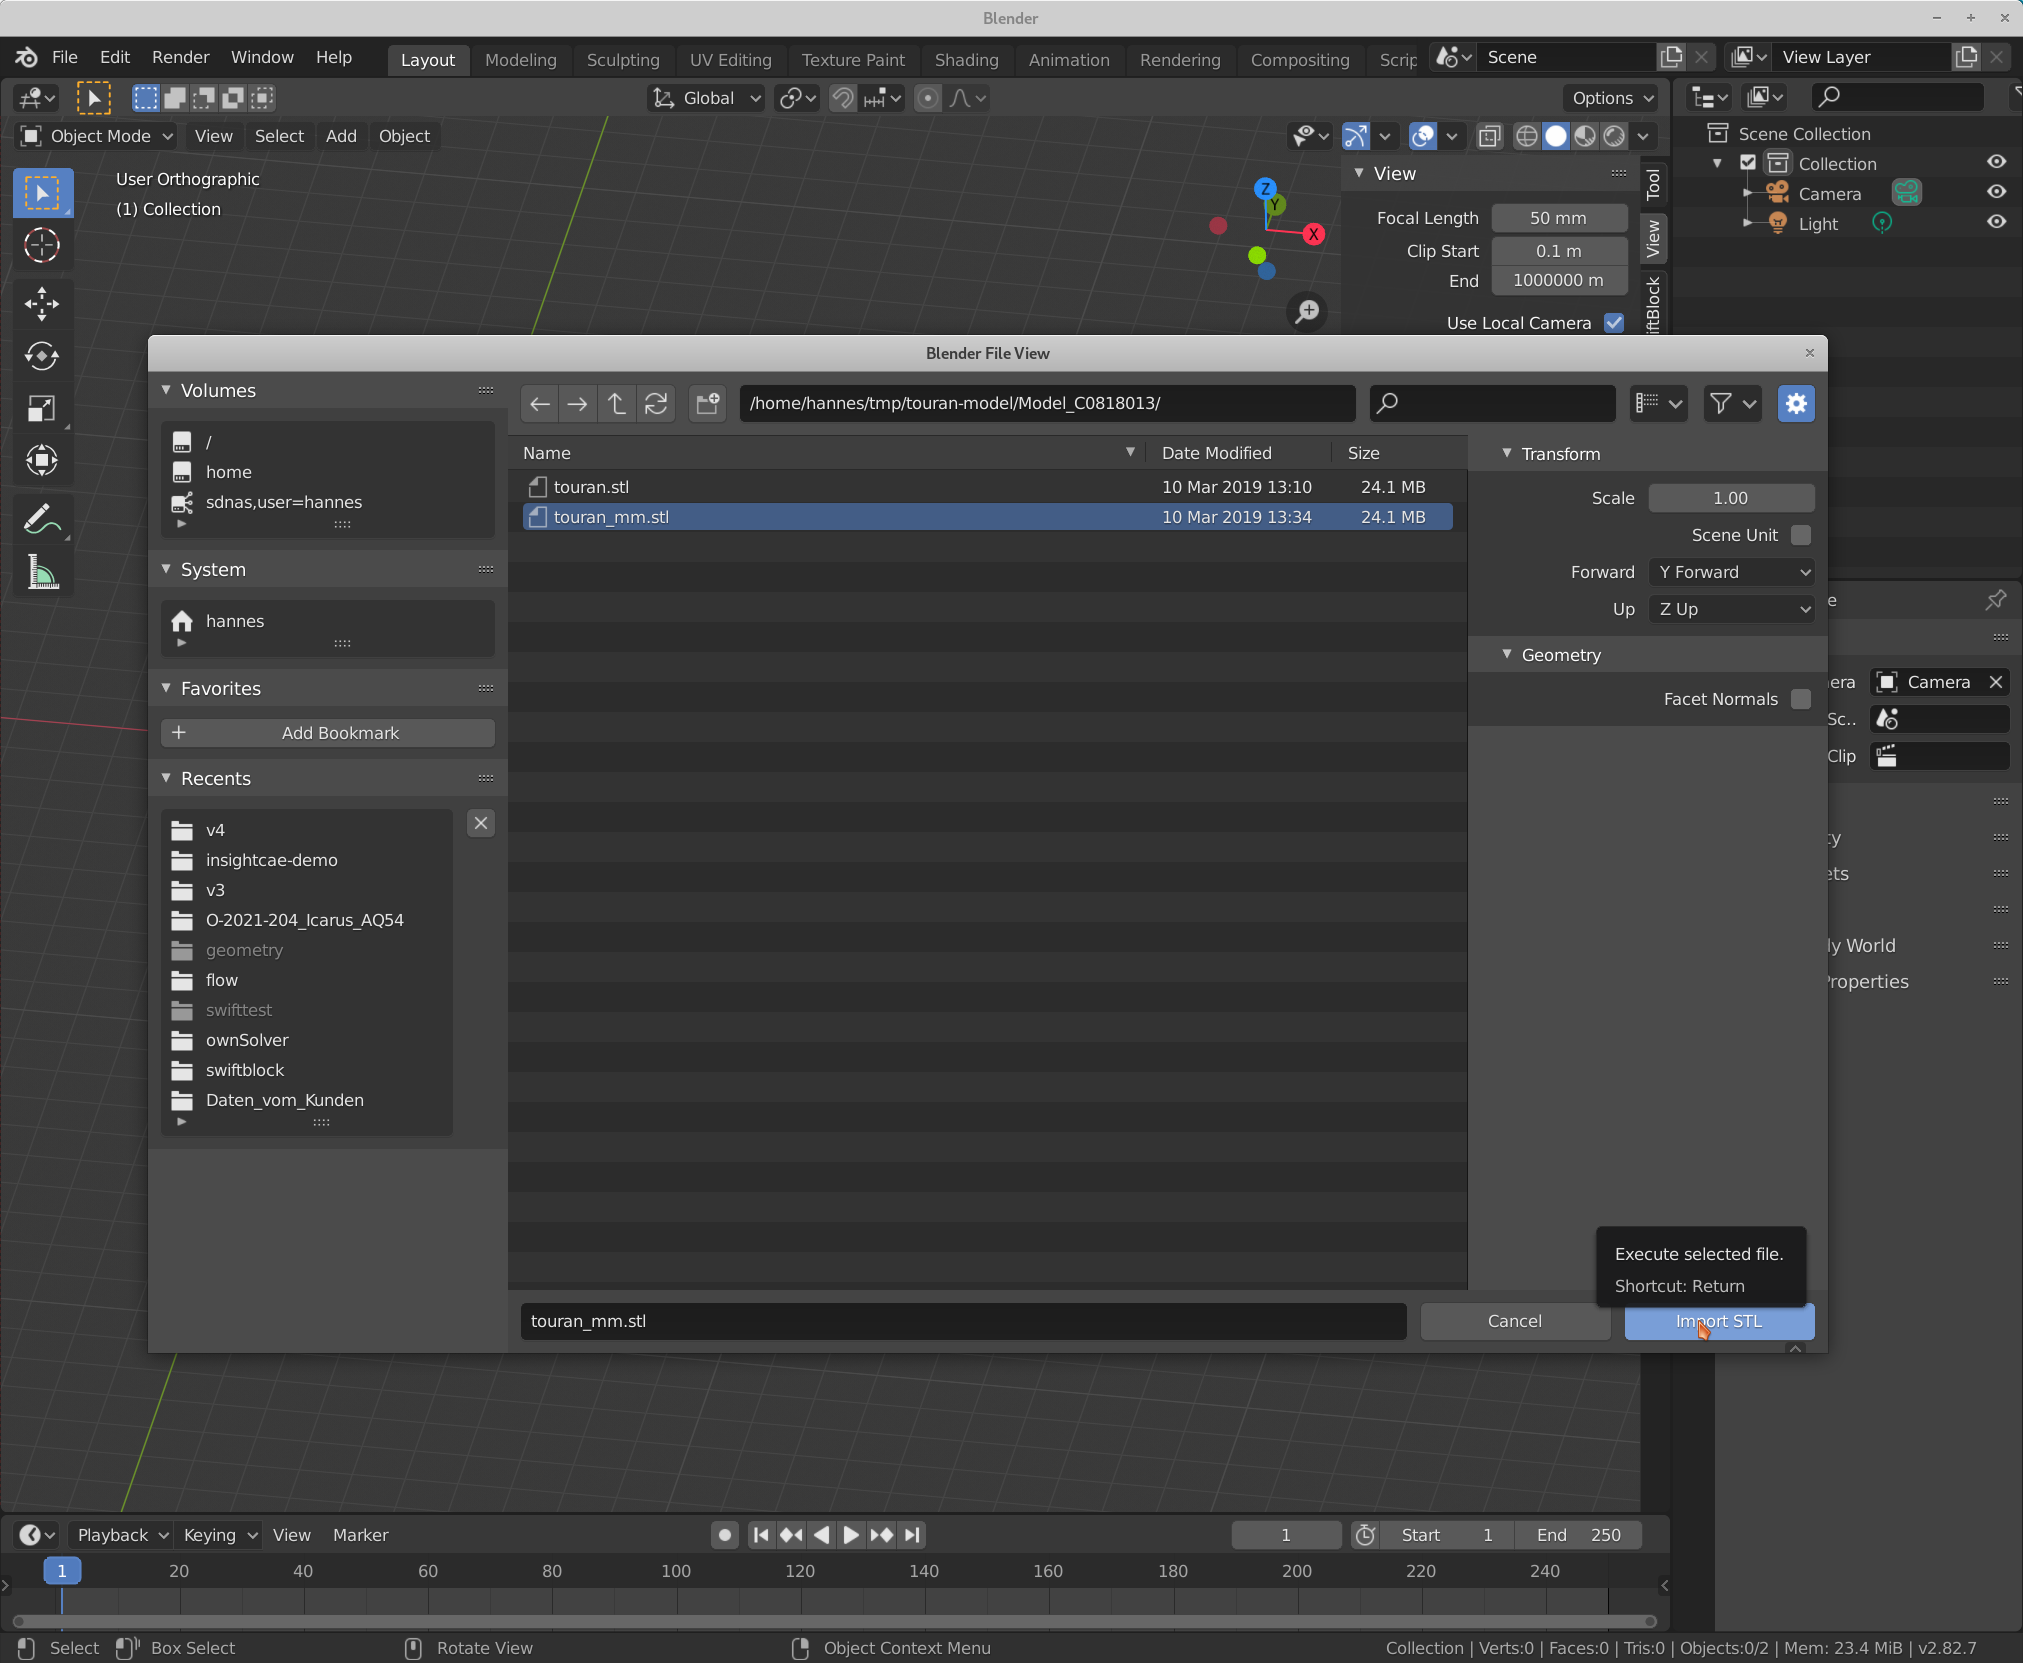
\includegraphics[width=0.75\linewidth]{figs/feature_edges_blender/02_import_stl_2}

\item make sure, the object is selected (orange line around the selected object is displayed)

Objects can be selected by left click them with mouse.

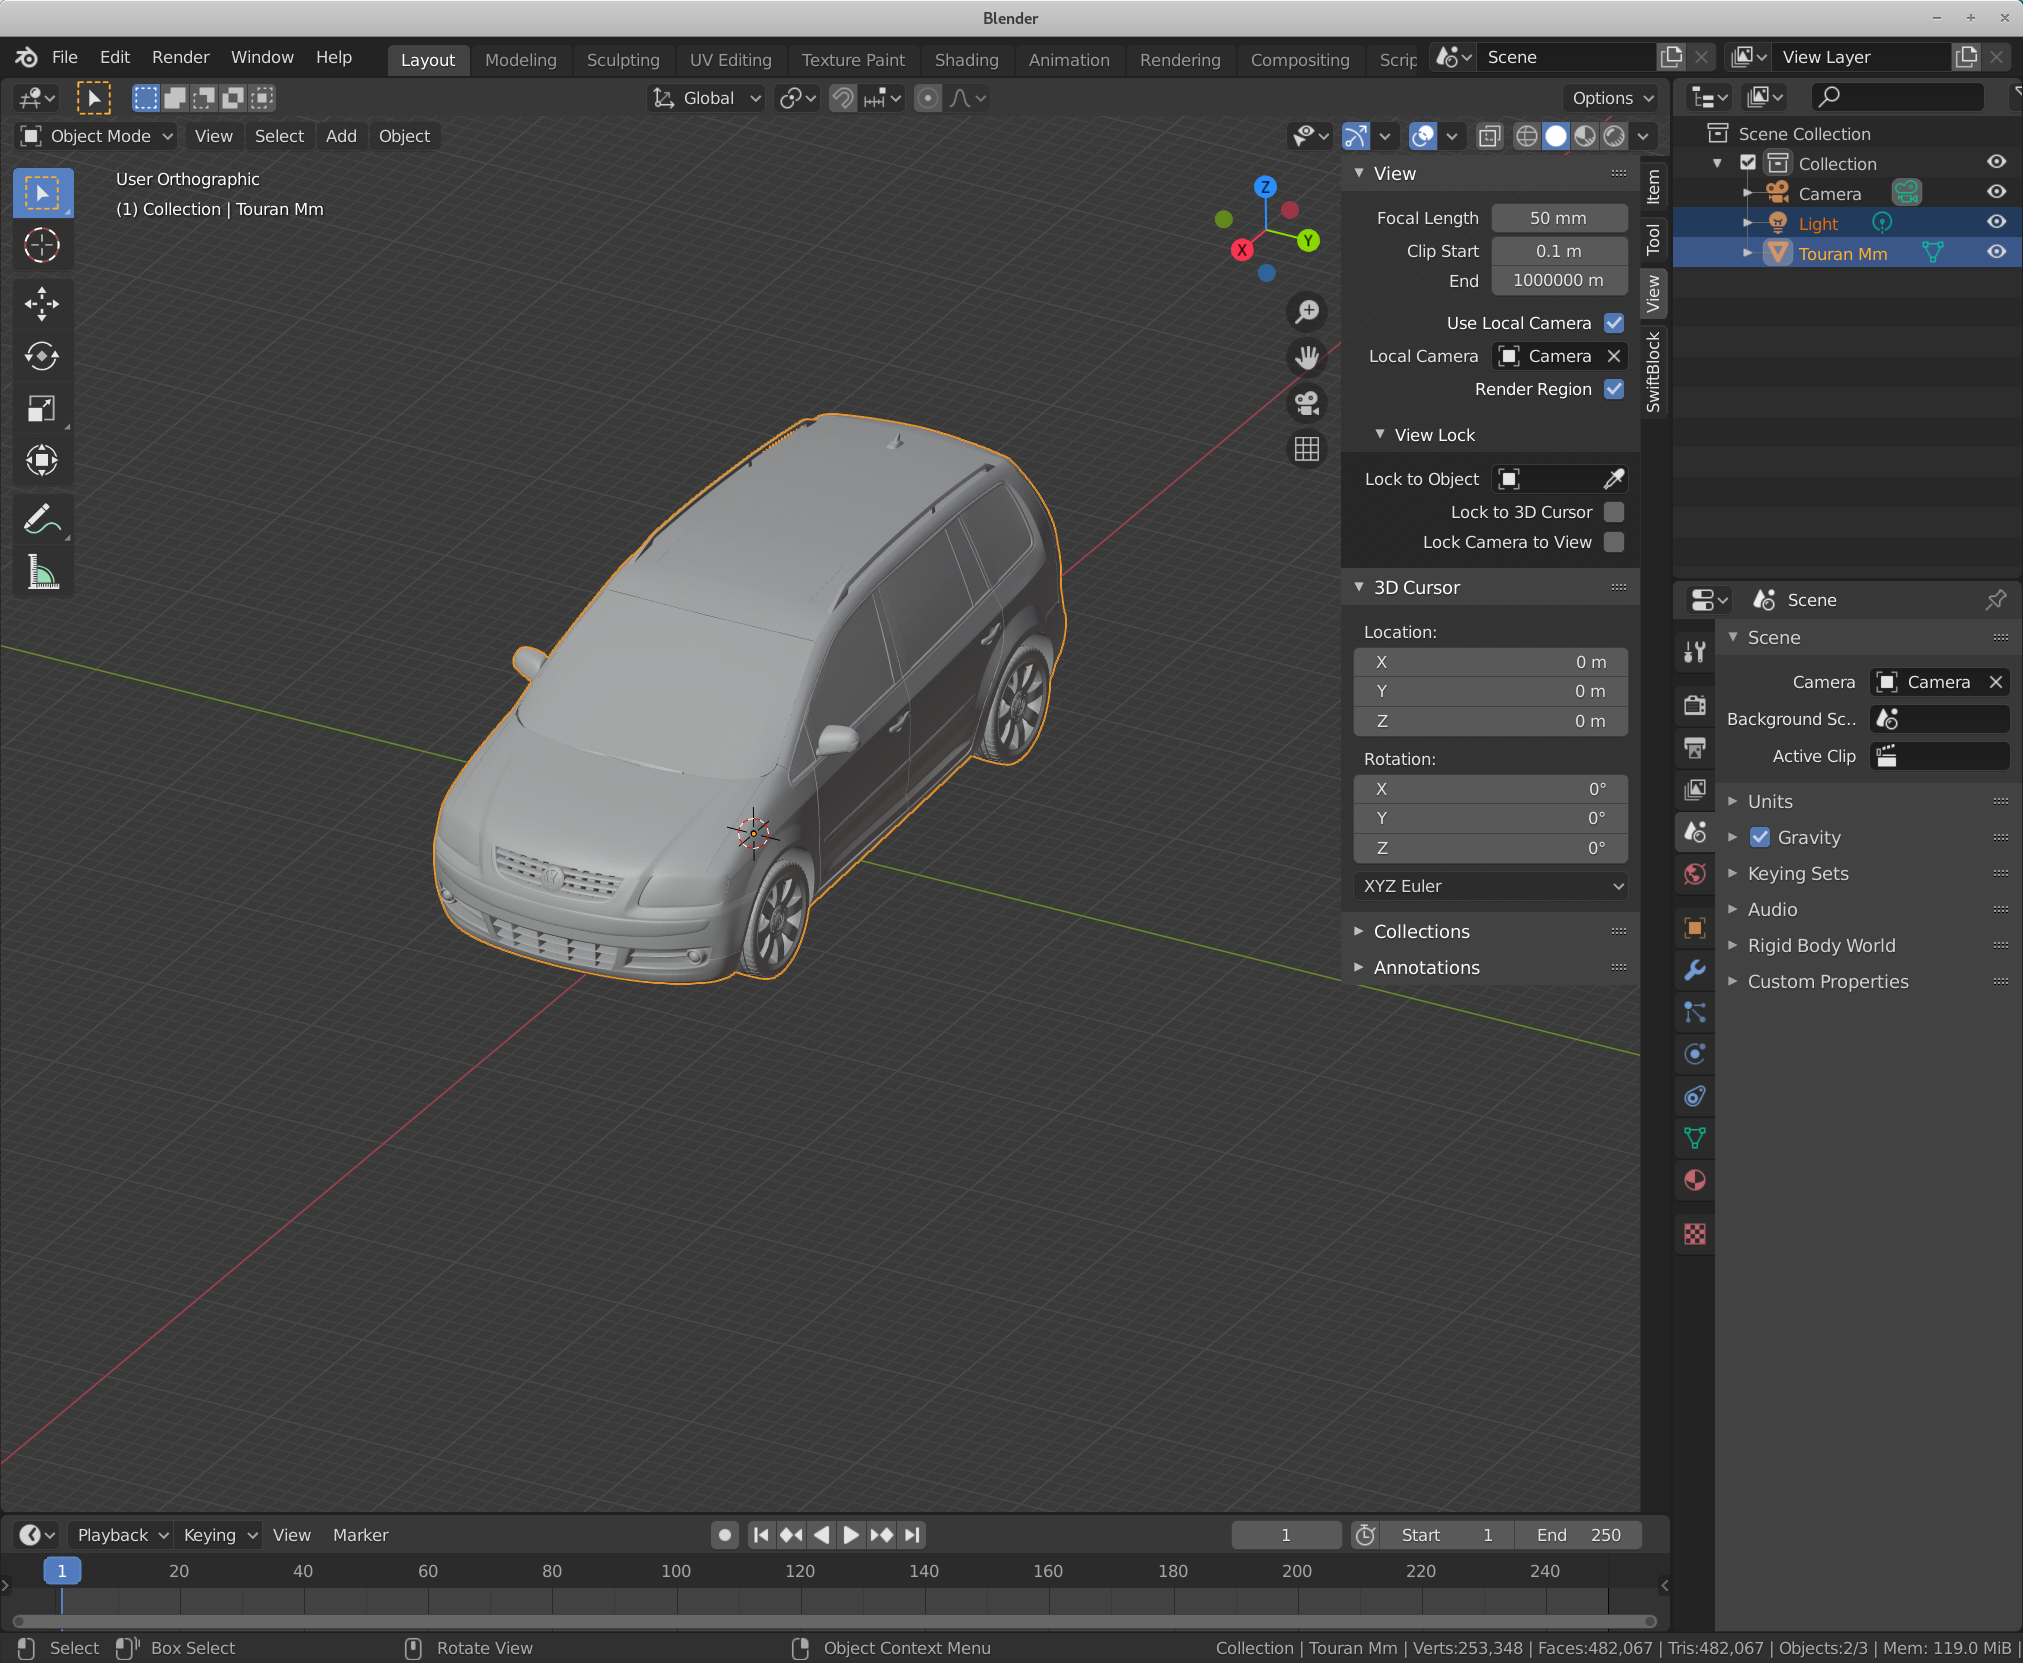
\includegraphics[width=0.75\linewidth]{figs/feature_edges_blender/03_stl_imported}

\item switch to "Edit Mode", either by pressing the "Tab" key or by selecting the mode in the combo box in the upper left corner.

Next, switch to edge selection mode (second button right from the edit mode combo box)

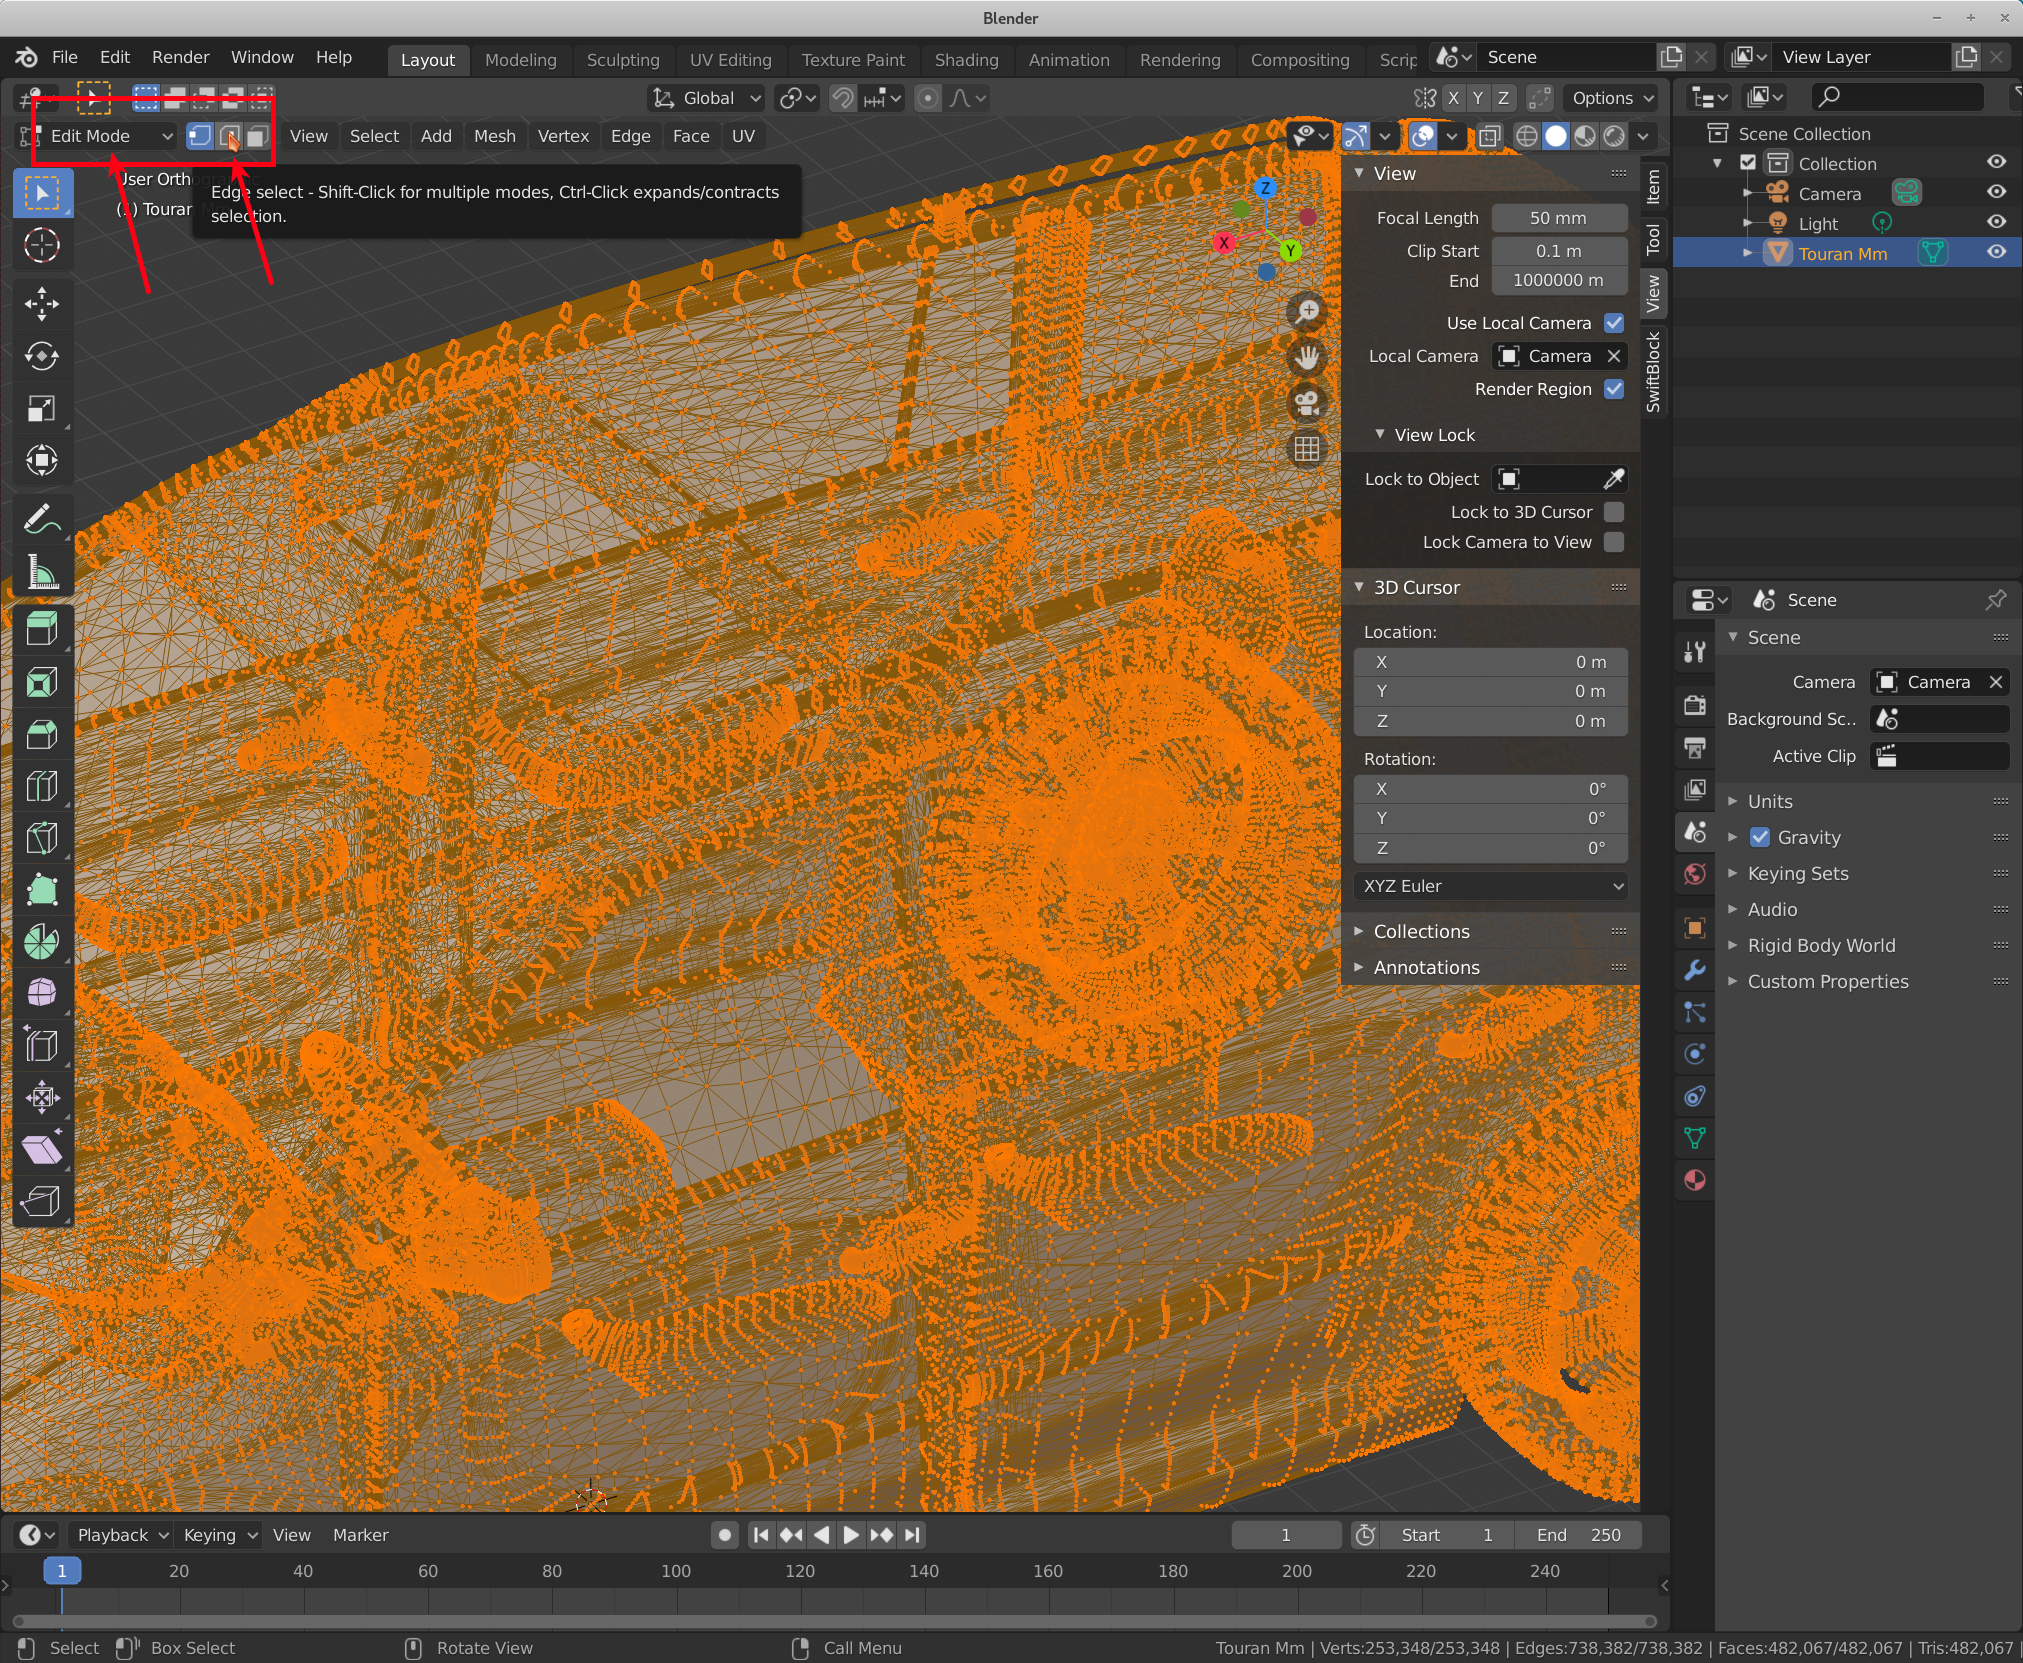
\includegraphics[width=0.75\linewidth]{figs/feature_edges_blender/04_edit_mode}

In this example, we want to select a line (chain of edges) along the left roof rail.

\item zoom into the location of the beginning of the line
\label{pt:begin_sel}

select the first edge with a left click on it.

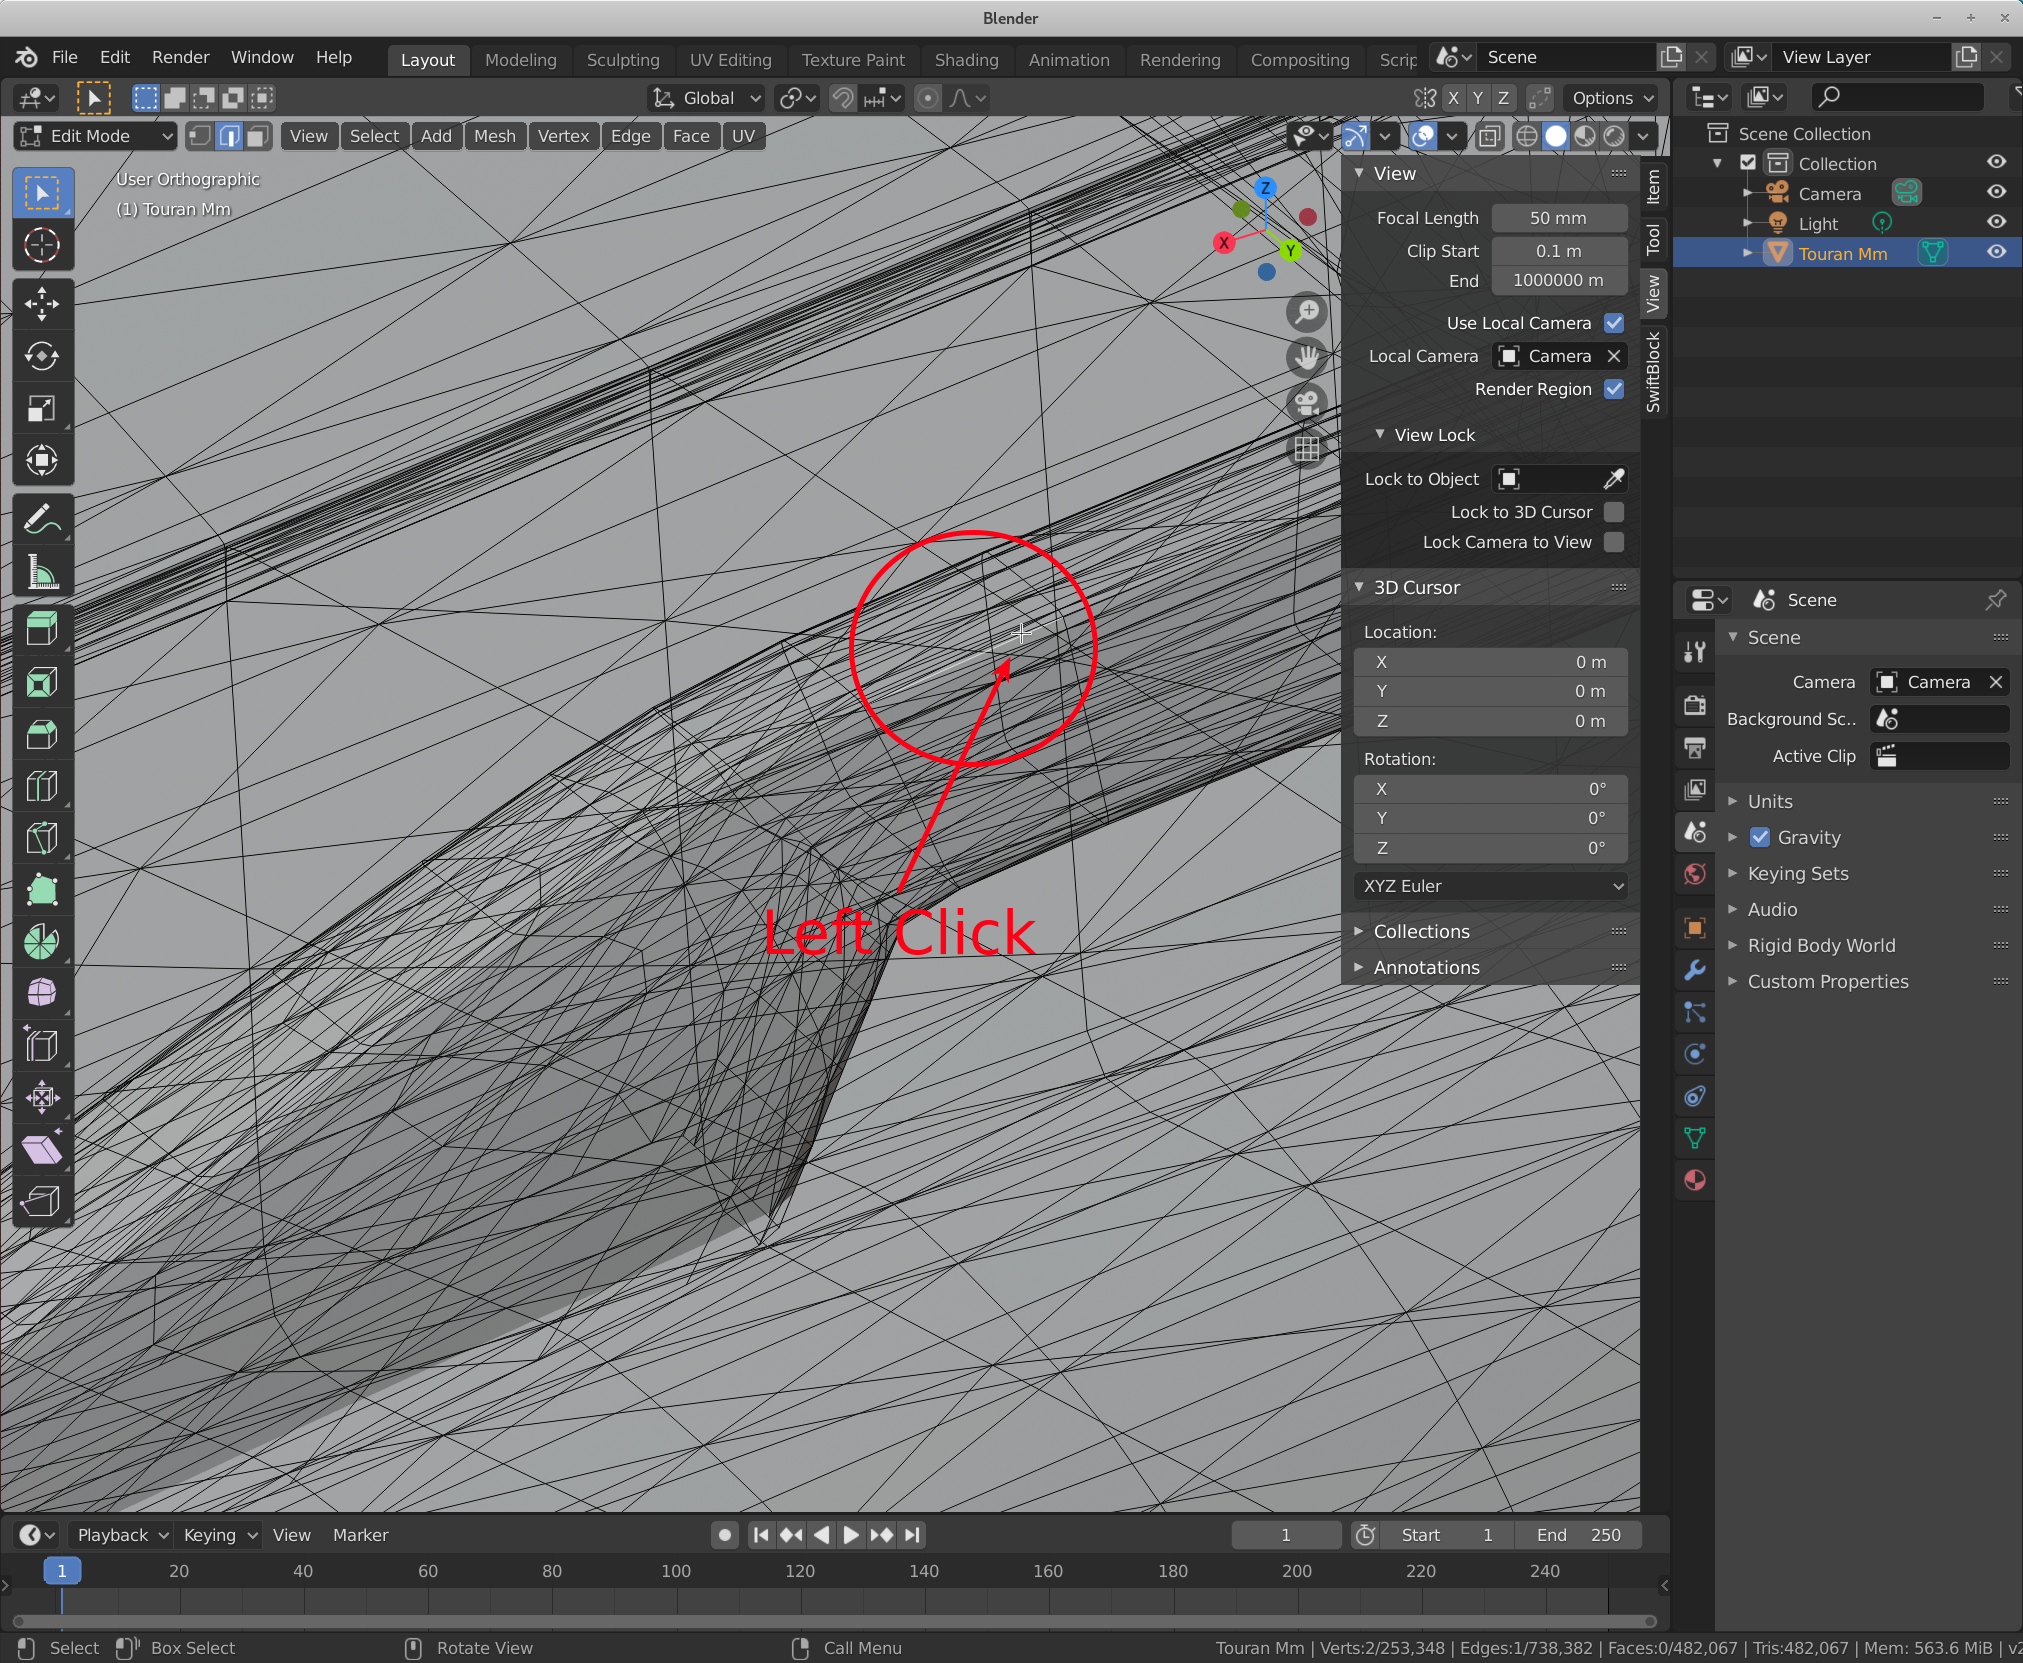
\includegraphics[width=0.75\linewidth]{figs/feature_edges_blender/05_select_first_edge}

\item select another edge on the feature line: zoom to the next location and press Ctrl + Left click

The shortest path from the last selected edge and the current clicked edge will be added to the selection.
To select edges as precise as possible, it might be required to click a number of intermediate locations.
If a mistake is made, the last step can be undone by typing Ctrl+Z.

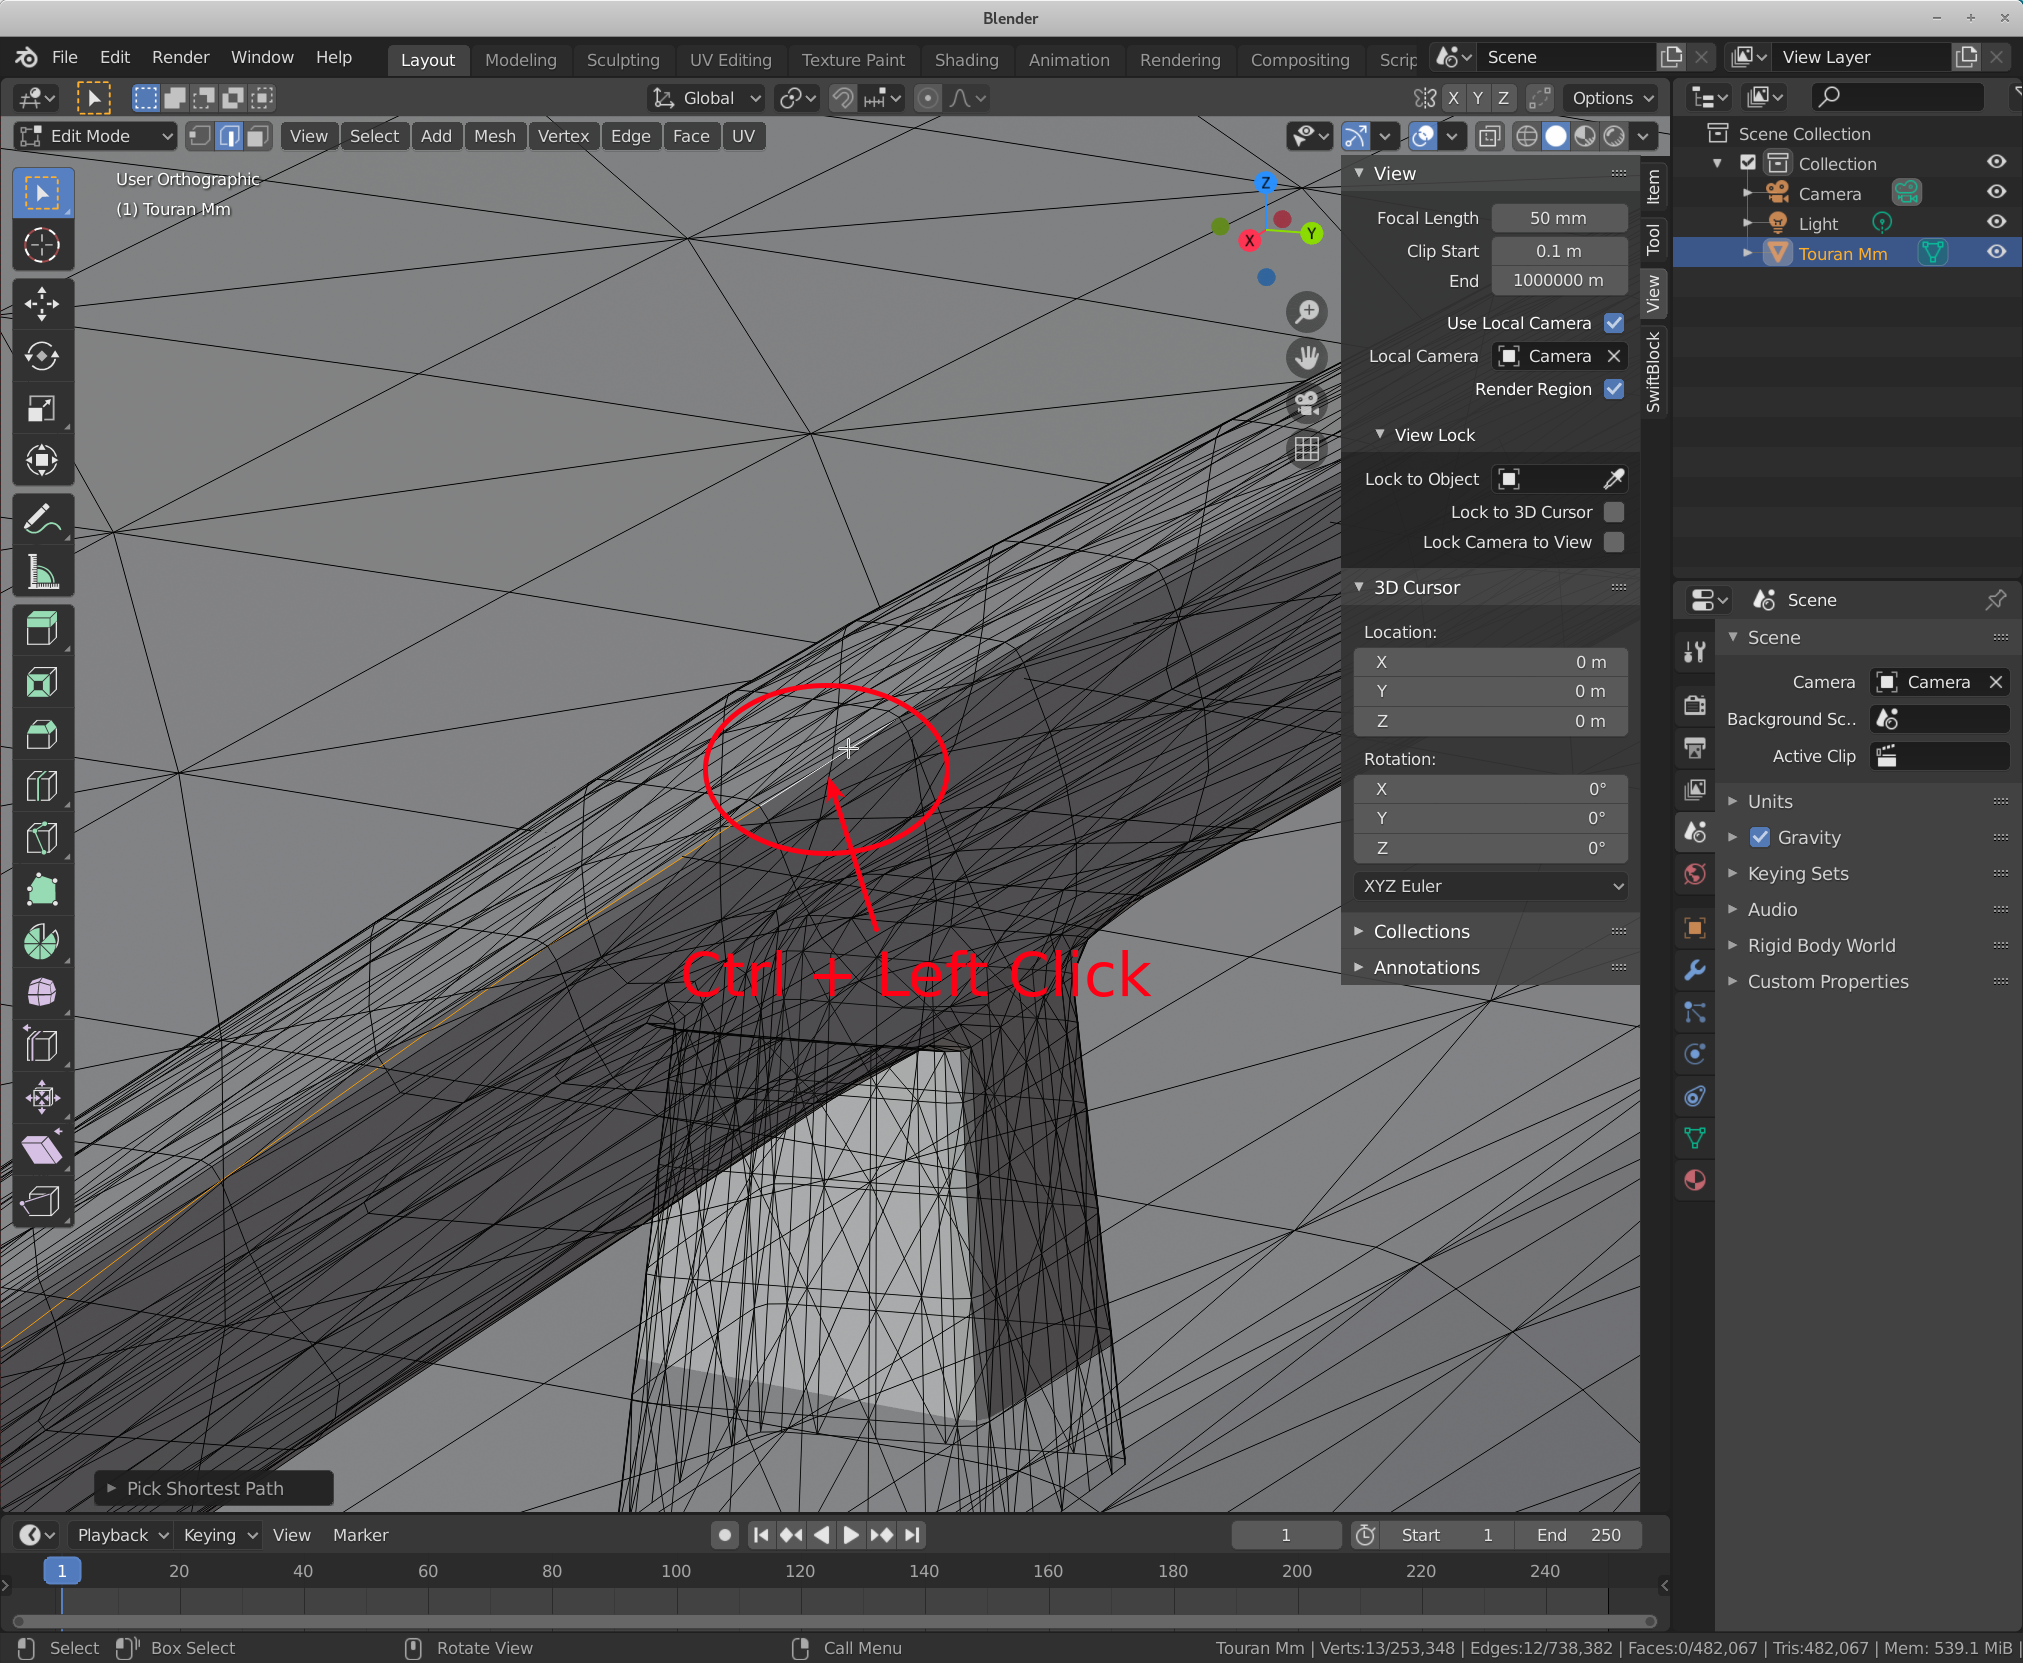
\includegraphics[width=0.75\linewidth]{figs/feature_edges_blender/06_select_second_edge}

\item repeat the last step until the end of the feature line is reached.

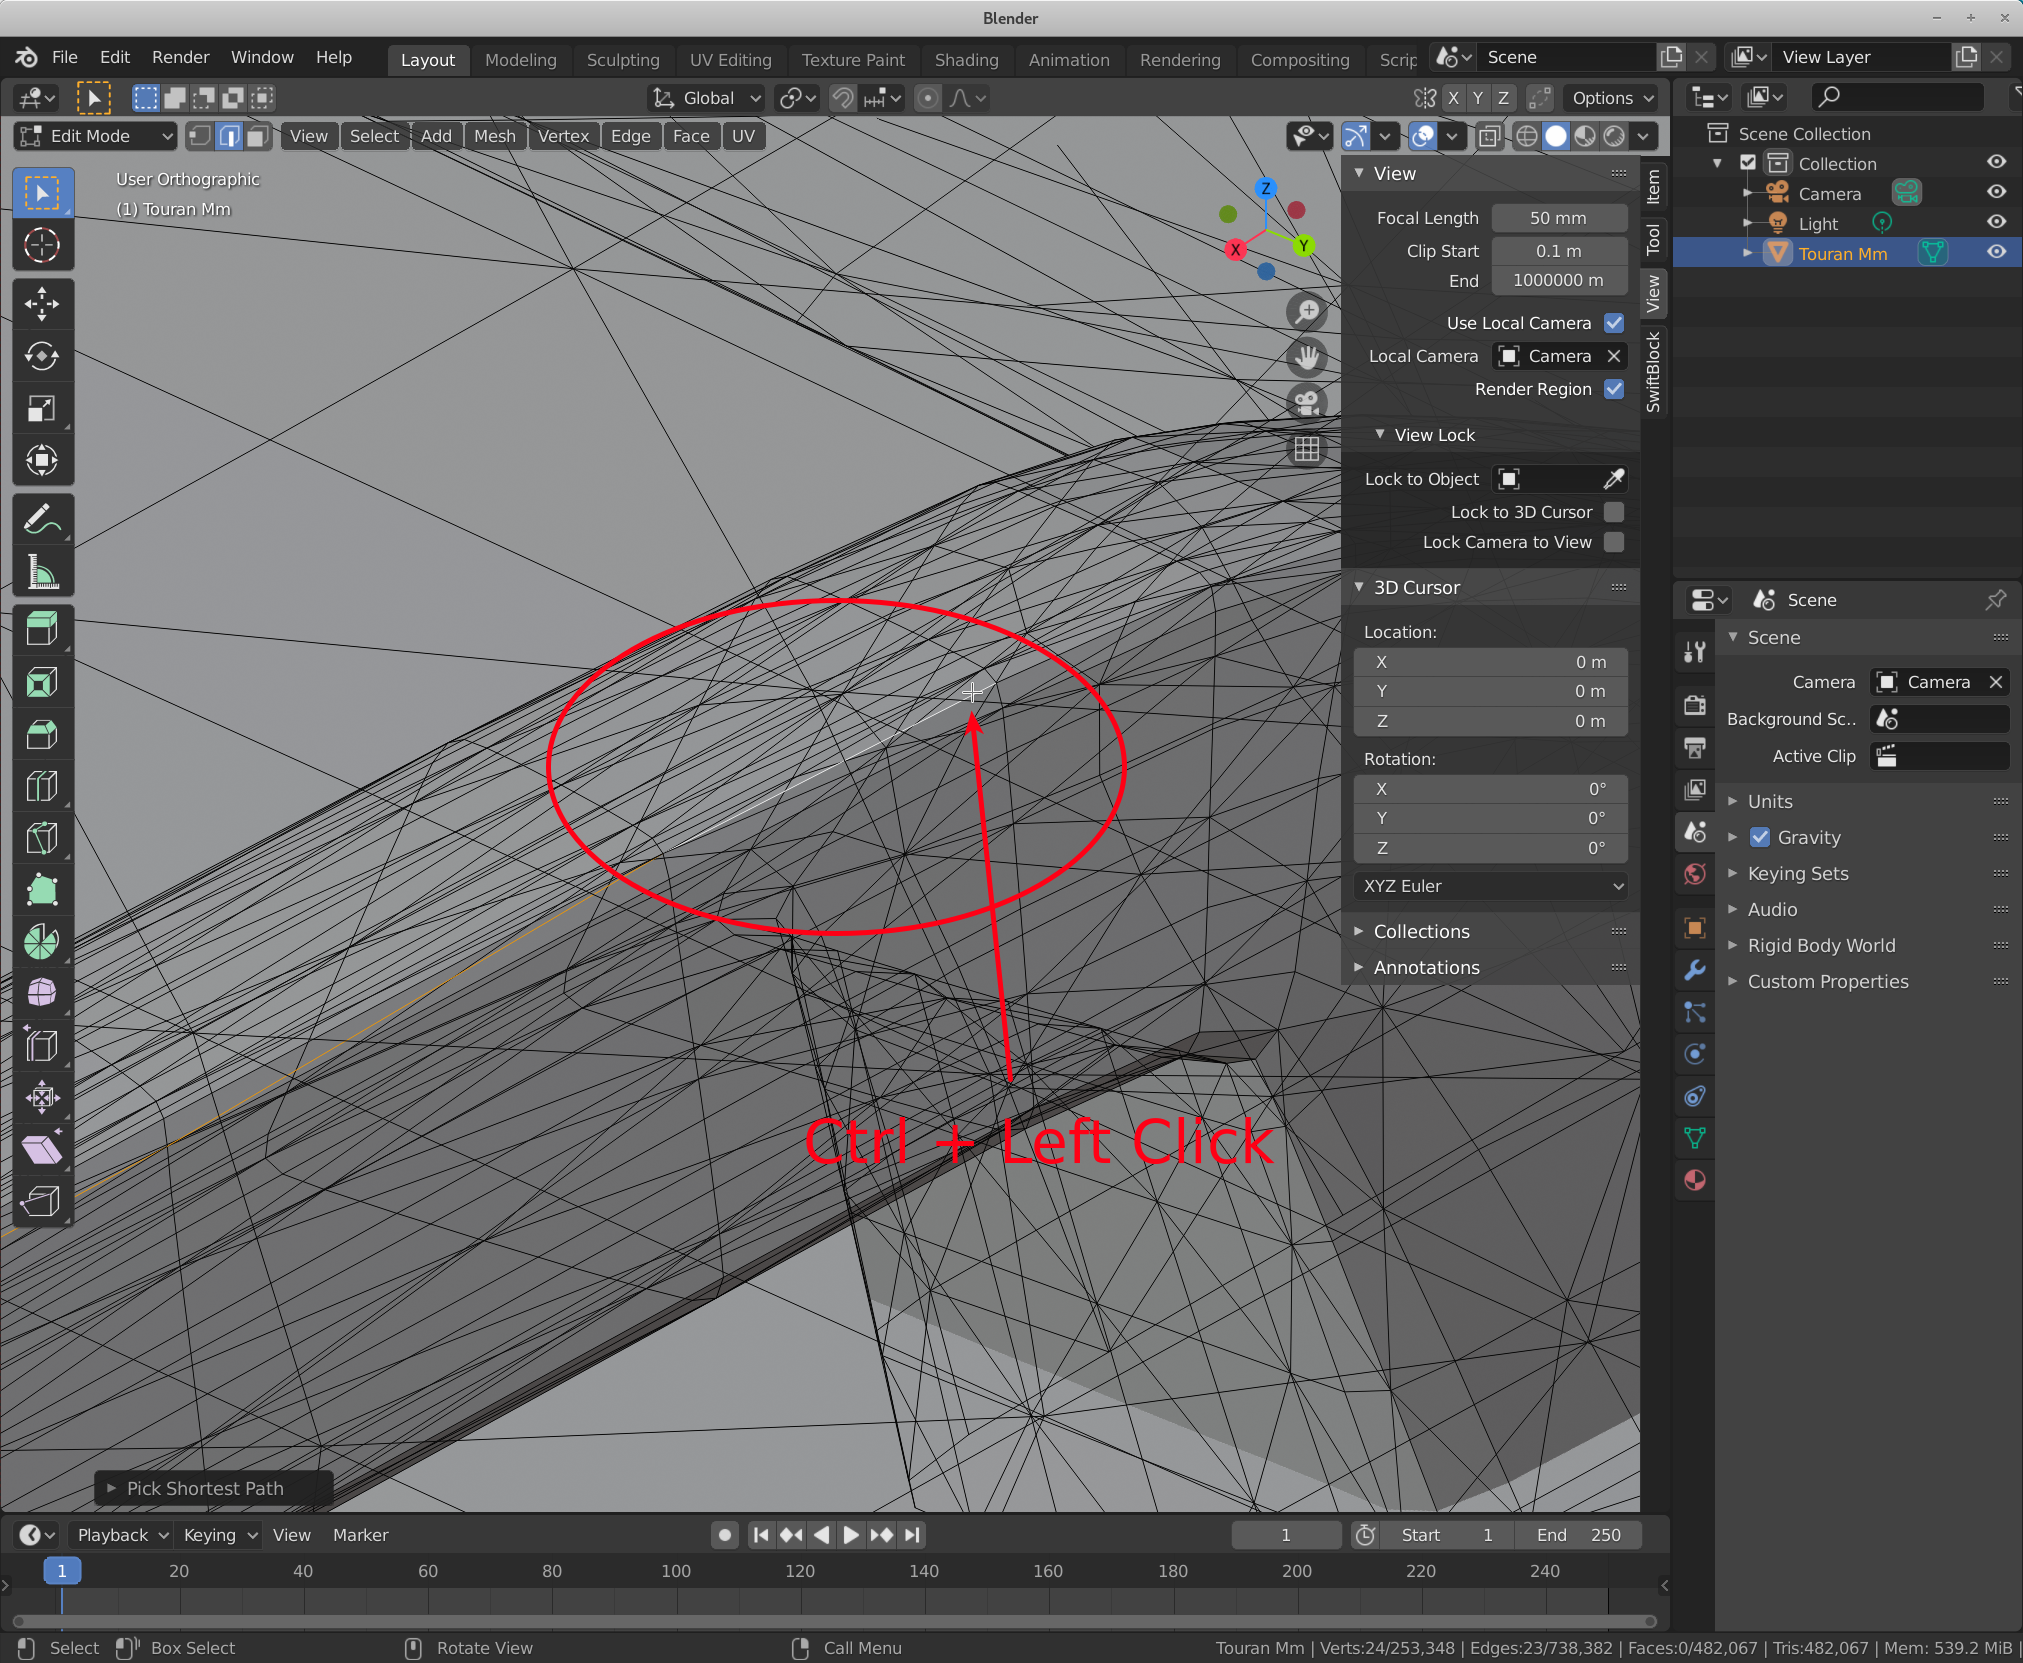
\includegraphics[width=0.75\linewidth]{figs/feature_edges_blender/07_select_last_edge}

\item next create a new object from the selected edges by typing the key "P".

Then select "Selection" to create the new part from the current selection.

Once the selection is split off, another chain of edges can be selected by repeating the steps from \ref{pt:begin_sel}.

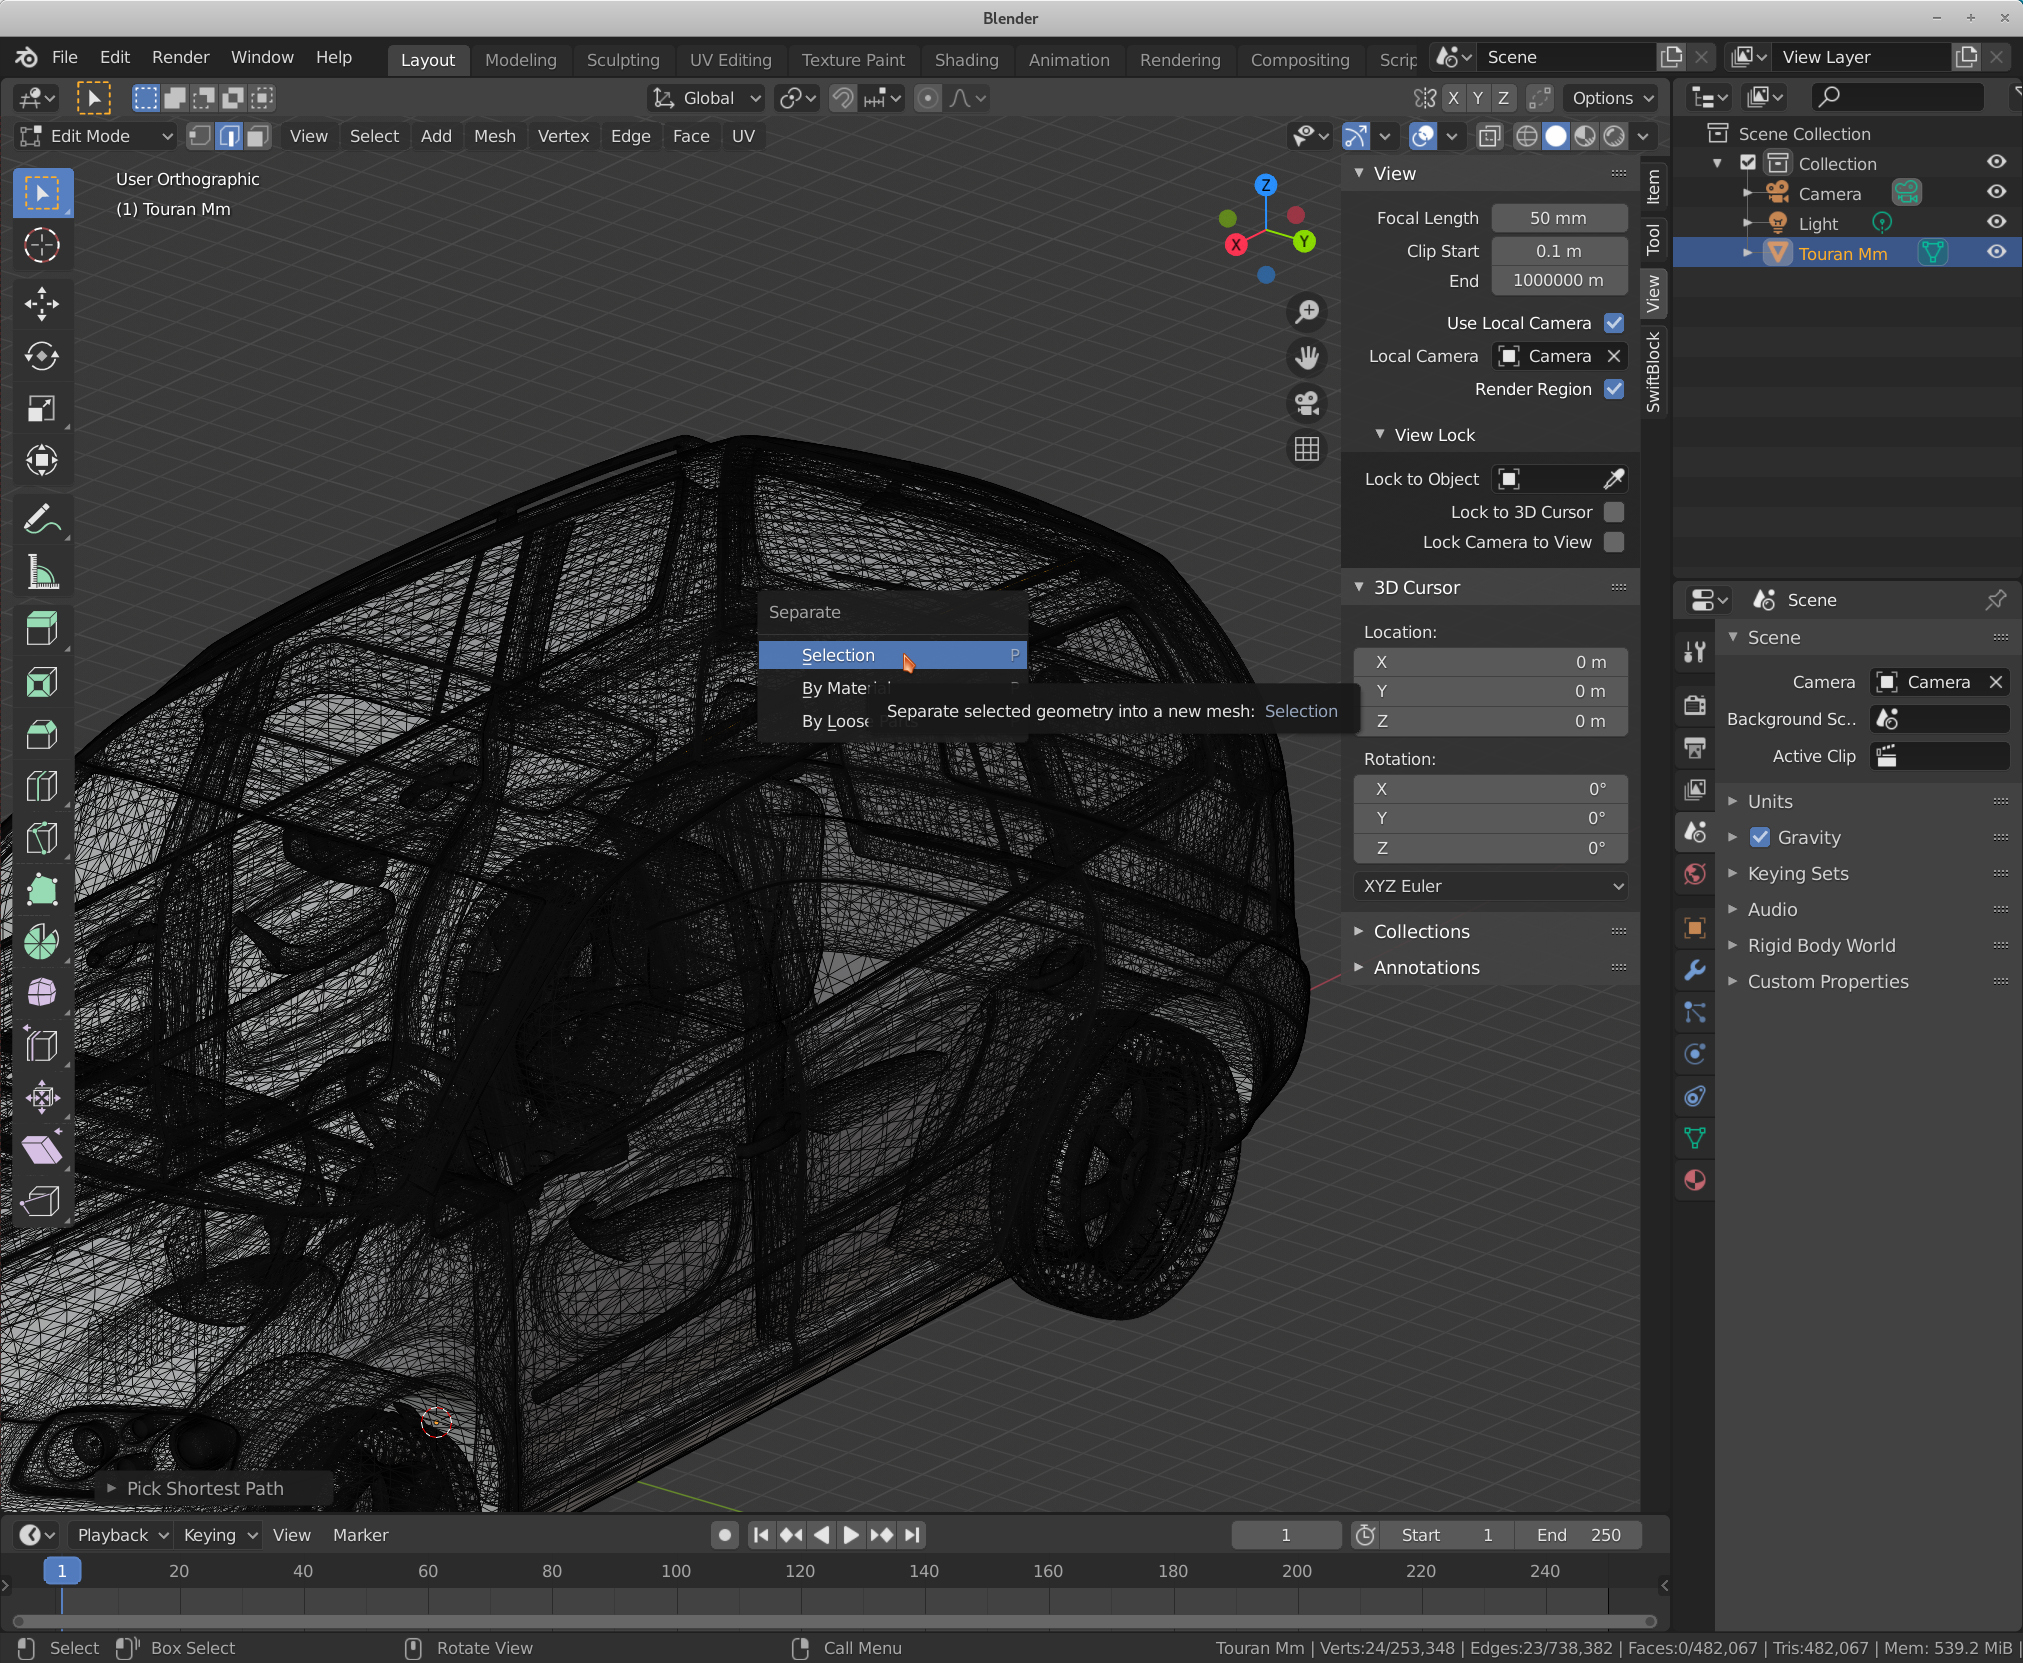
\includegraphics[width=0.75\linewidth]{figs/feature_edges_blender/08_export_selection}

\item switch back to "Object Mode"

either by pressing the Tab key or by selecting "Object Mode" in the combo box in the upper left corner.

When multiple lines had been split into multiple new objects, these should be joined into a single one.
To do so, select the objects in the object browser (upper right), then type "Ctrl+J".

Note: the mouse should be over the 3D viewport for Blender to accept the keyboard shortcut.

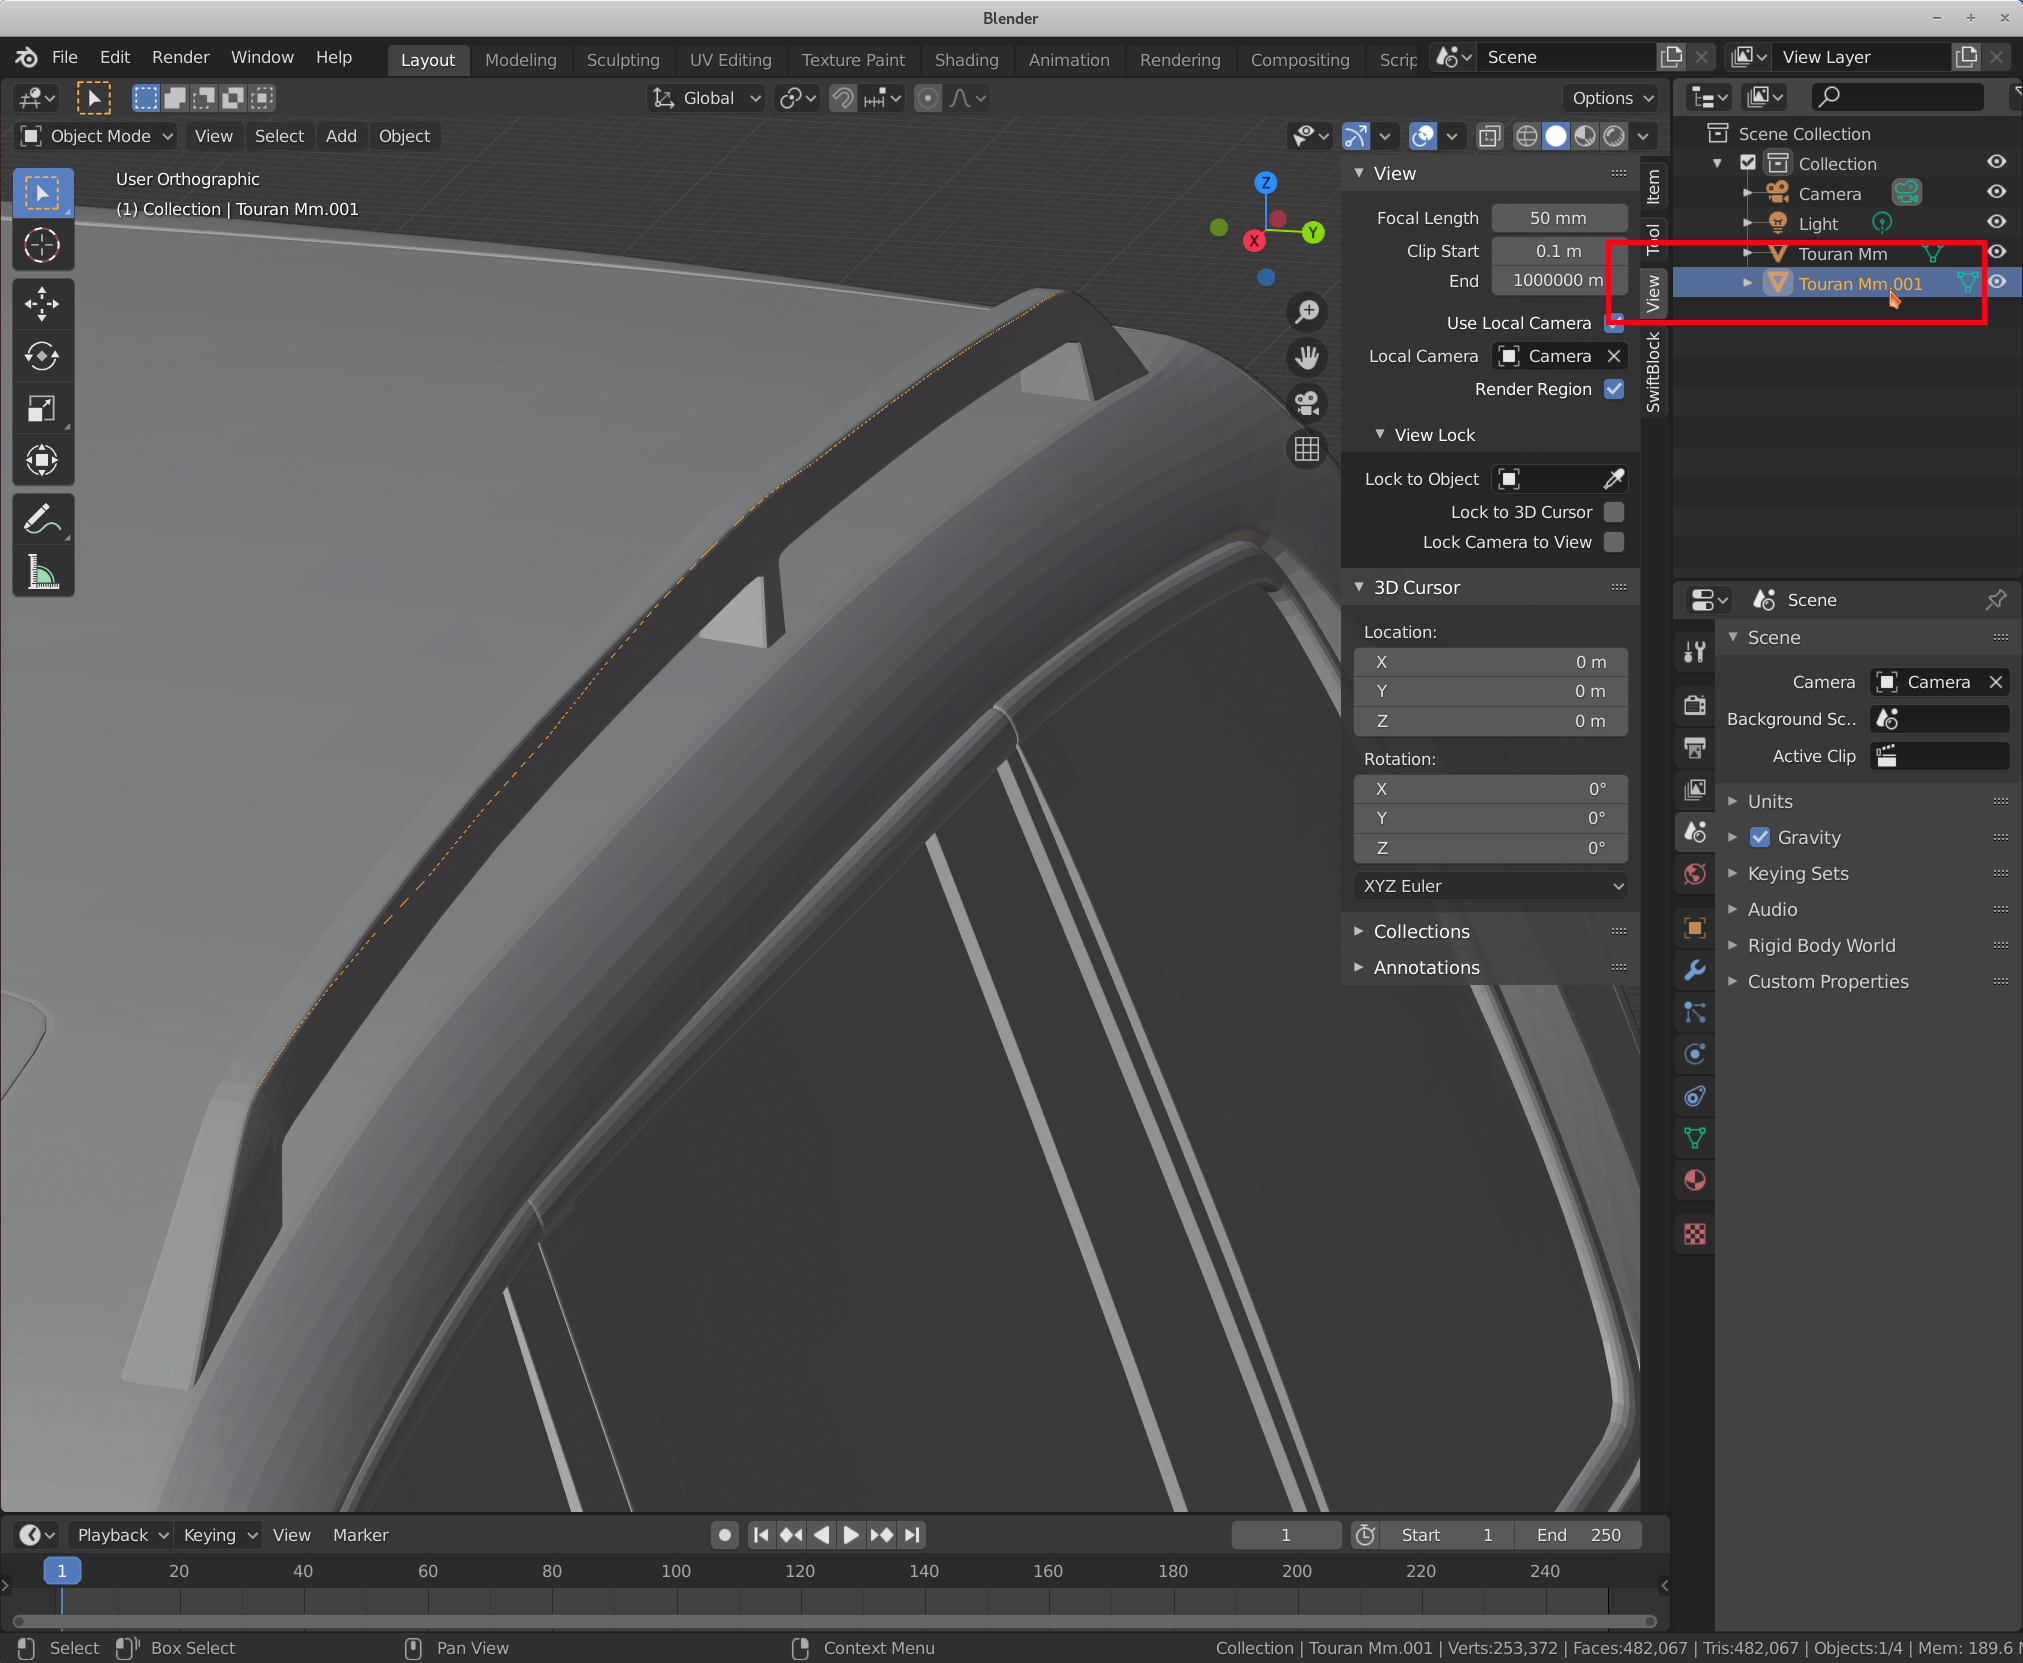
\includegraphics[width=0.75\linewidth]{figs/feature_edges_blender/09_view_result}

\item export the edges into an OBJ file.

Select the object in the object browser with a left click.

Then open the menu \menu{File>Export>Wavefront (*.obj)}.

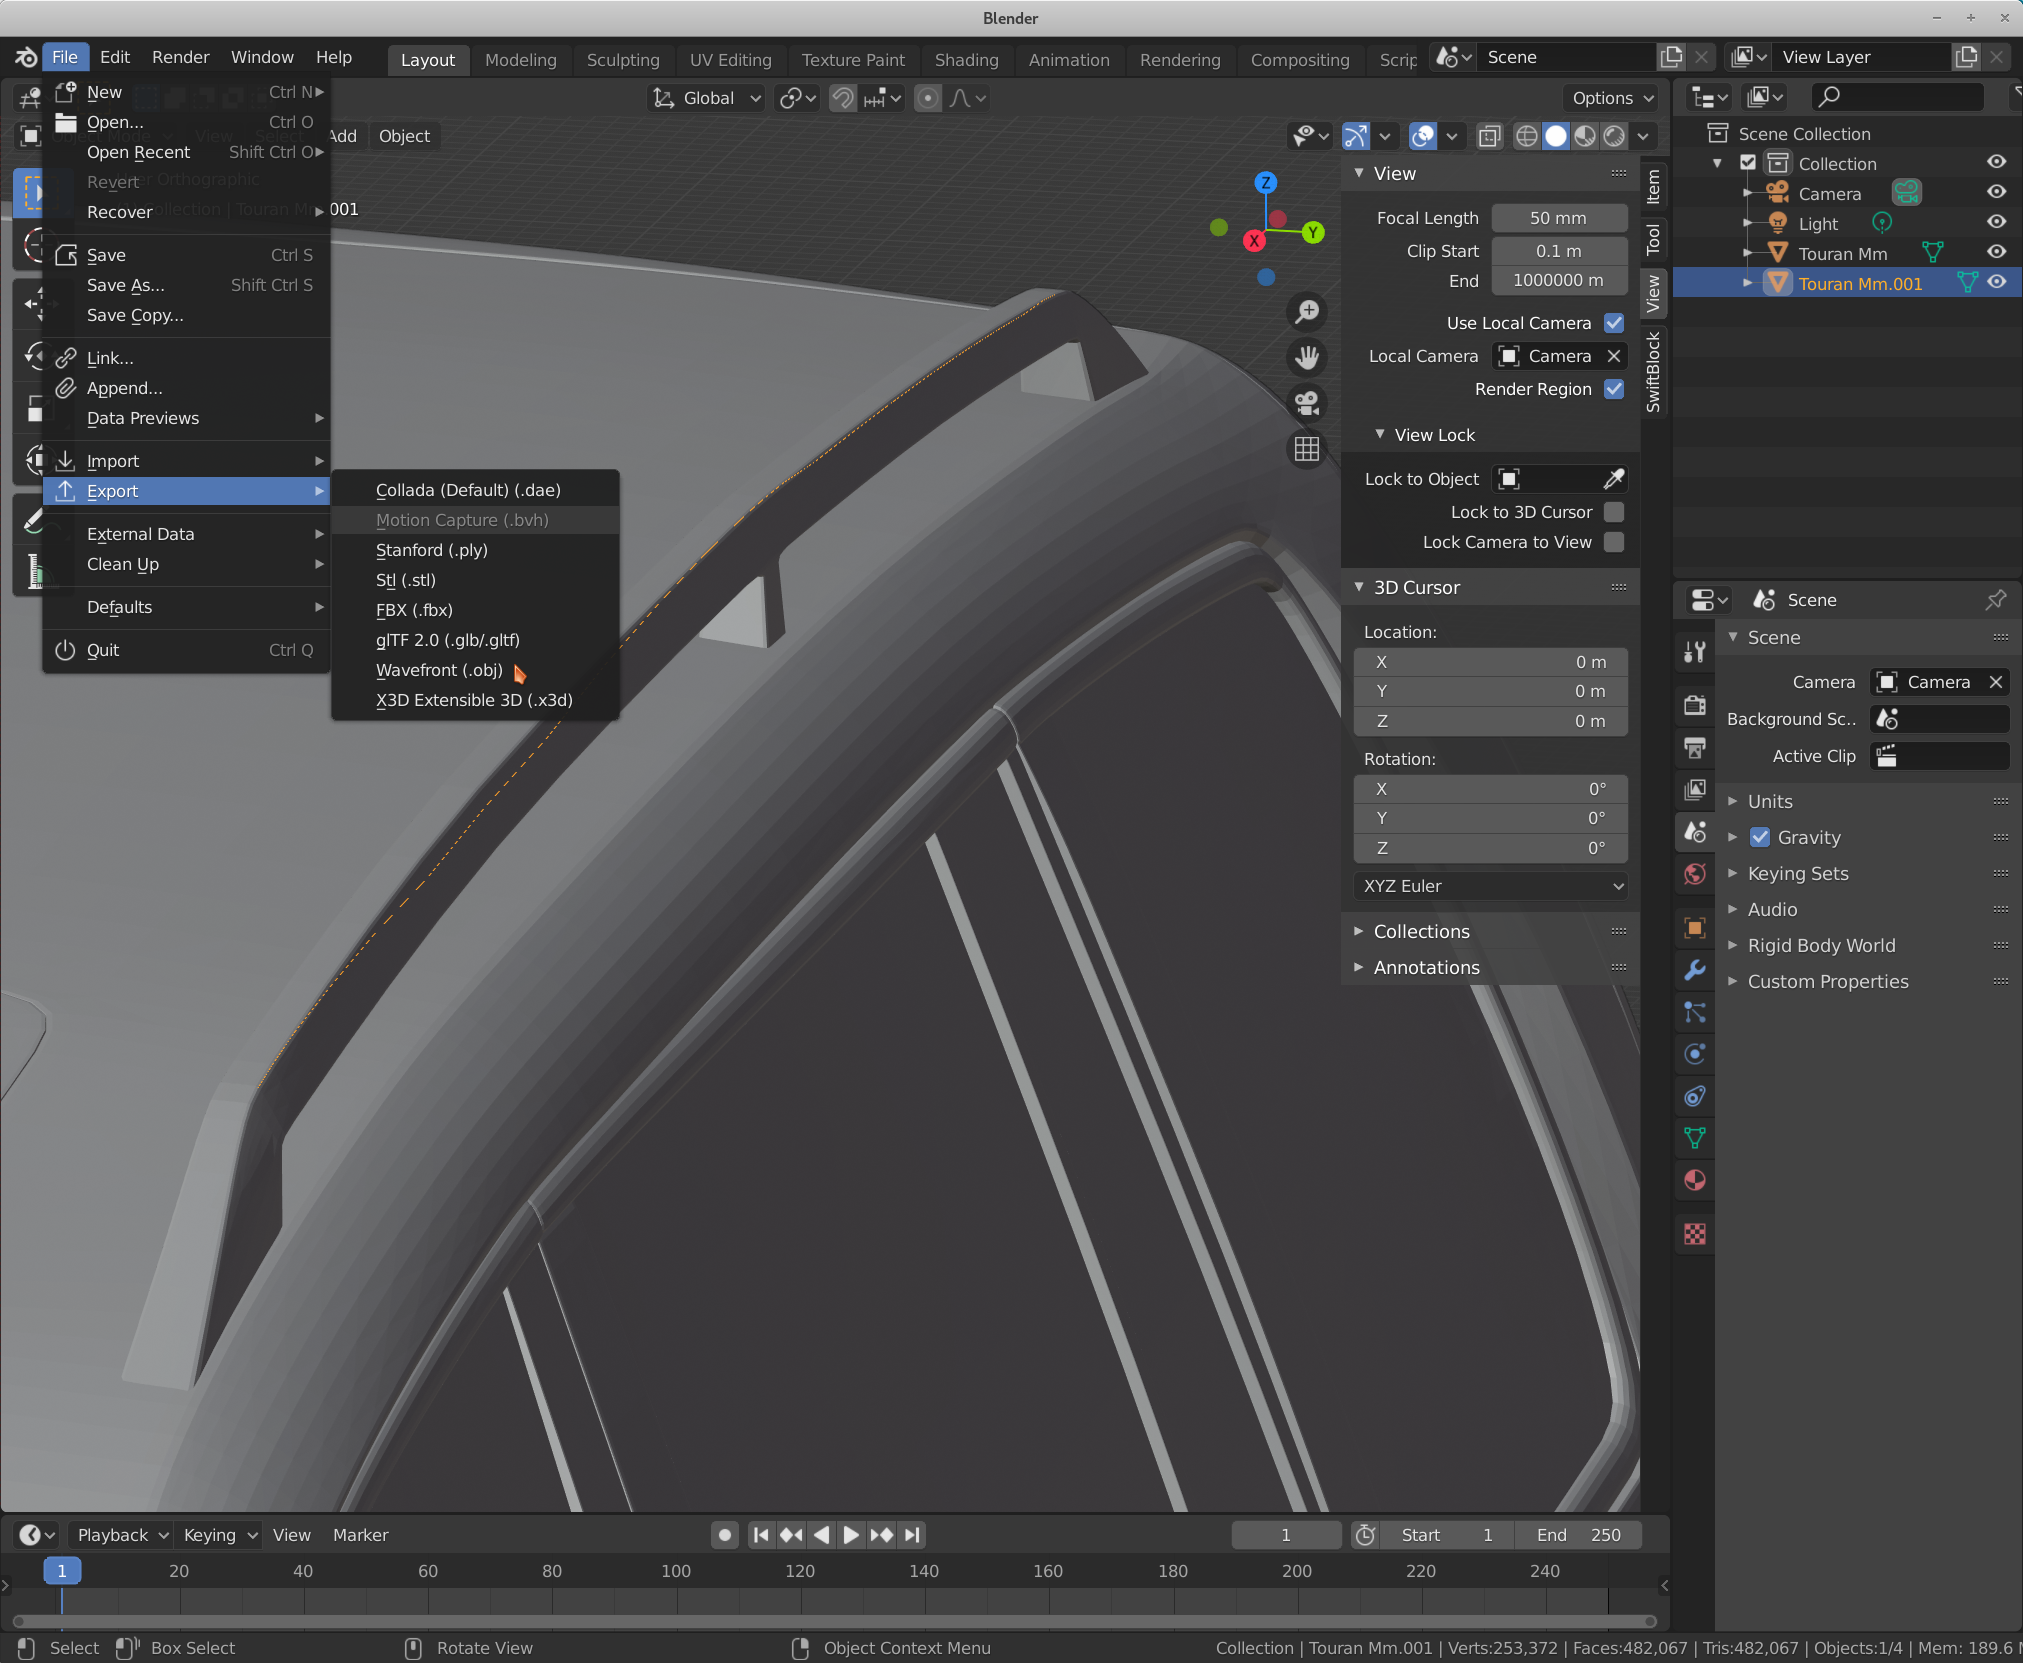
\includegraphics[width=0.75\linewidth]{figs/feature_edges_blender/10_export_obj}

\item check the export settings. Make sure, the following is set:

\begin{itemize}
\item "Selection only" is checked

(Otherwise also the surface will be included in the exported file)
\item In "Transform", "Forward" is set to "Y Forward"

(Otherwise the geometry will be wrongly oriented after export)
\end{itemize}


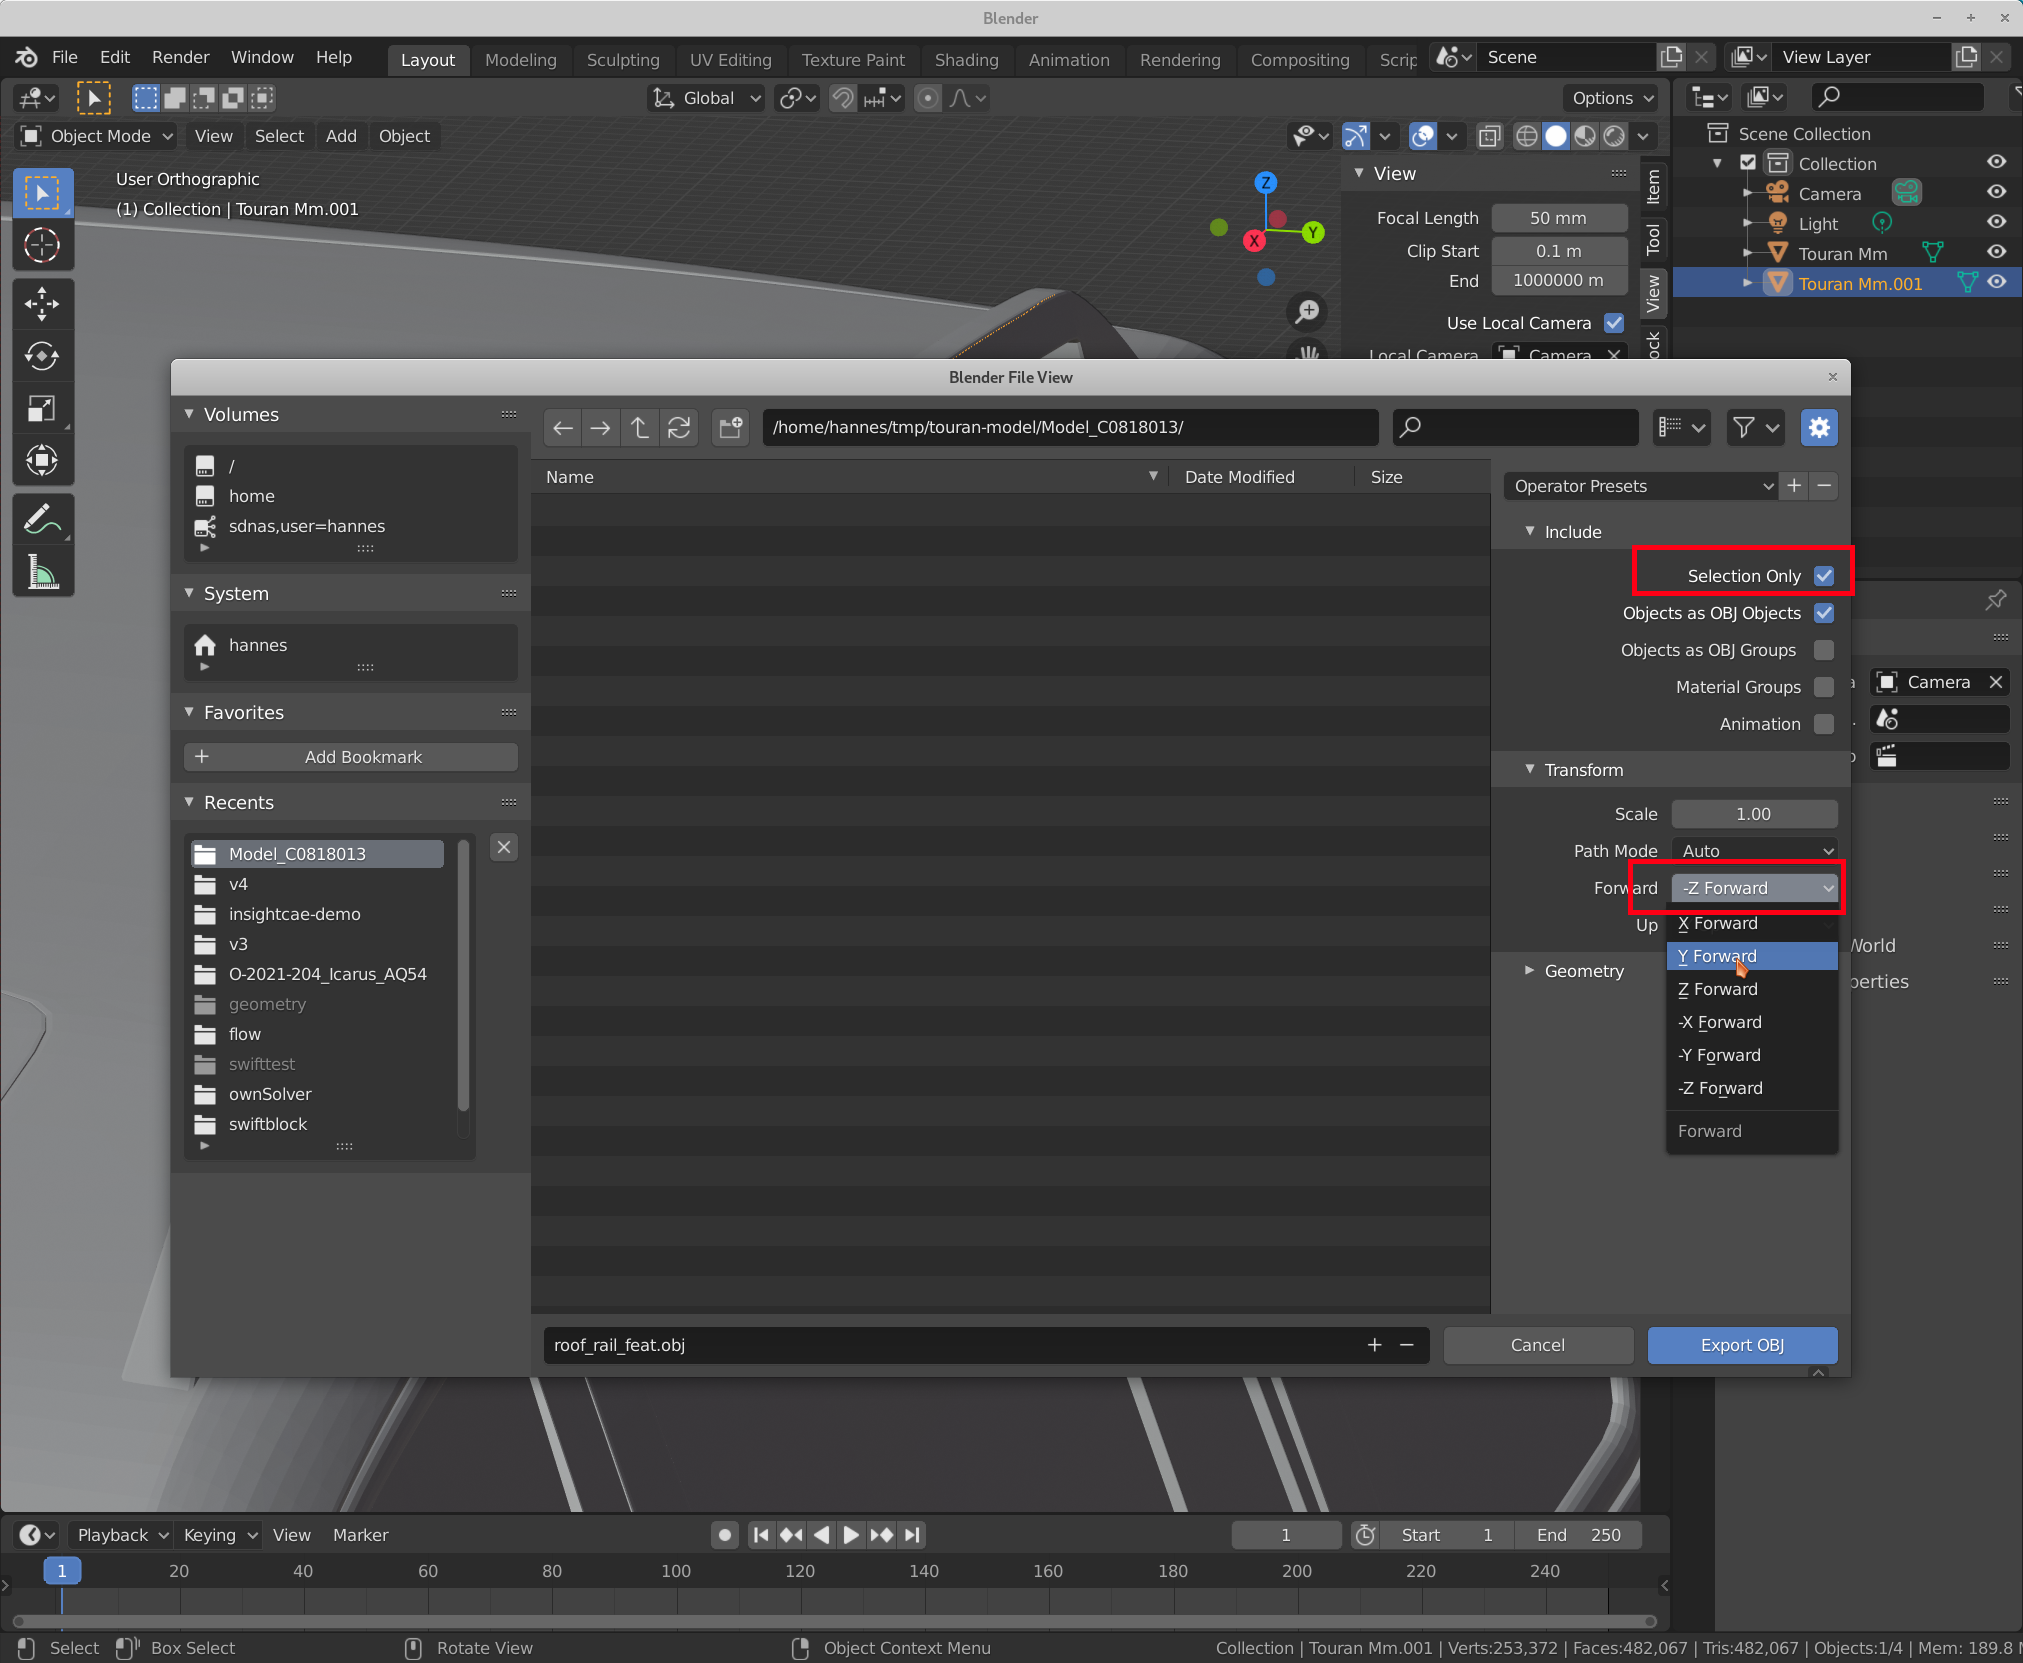
\includegraphics[width=0.75\linewidth]{figs/feature_edges_blender/11_export_setup}

\item the resulting OBJ files can be loaded into Paraview and checked

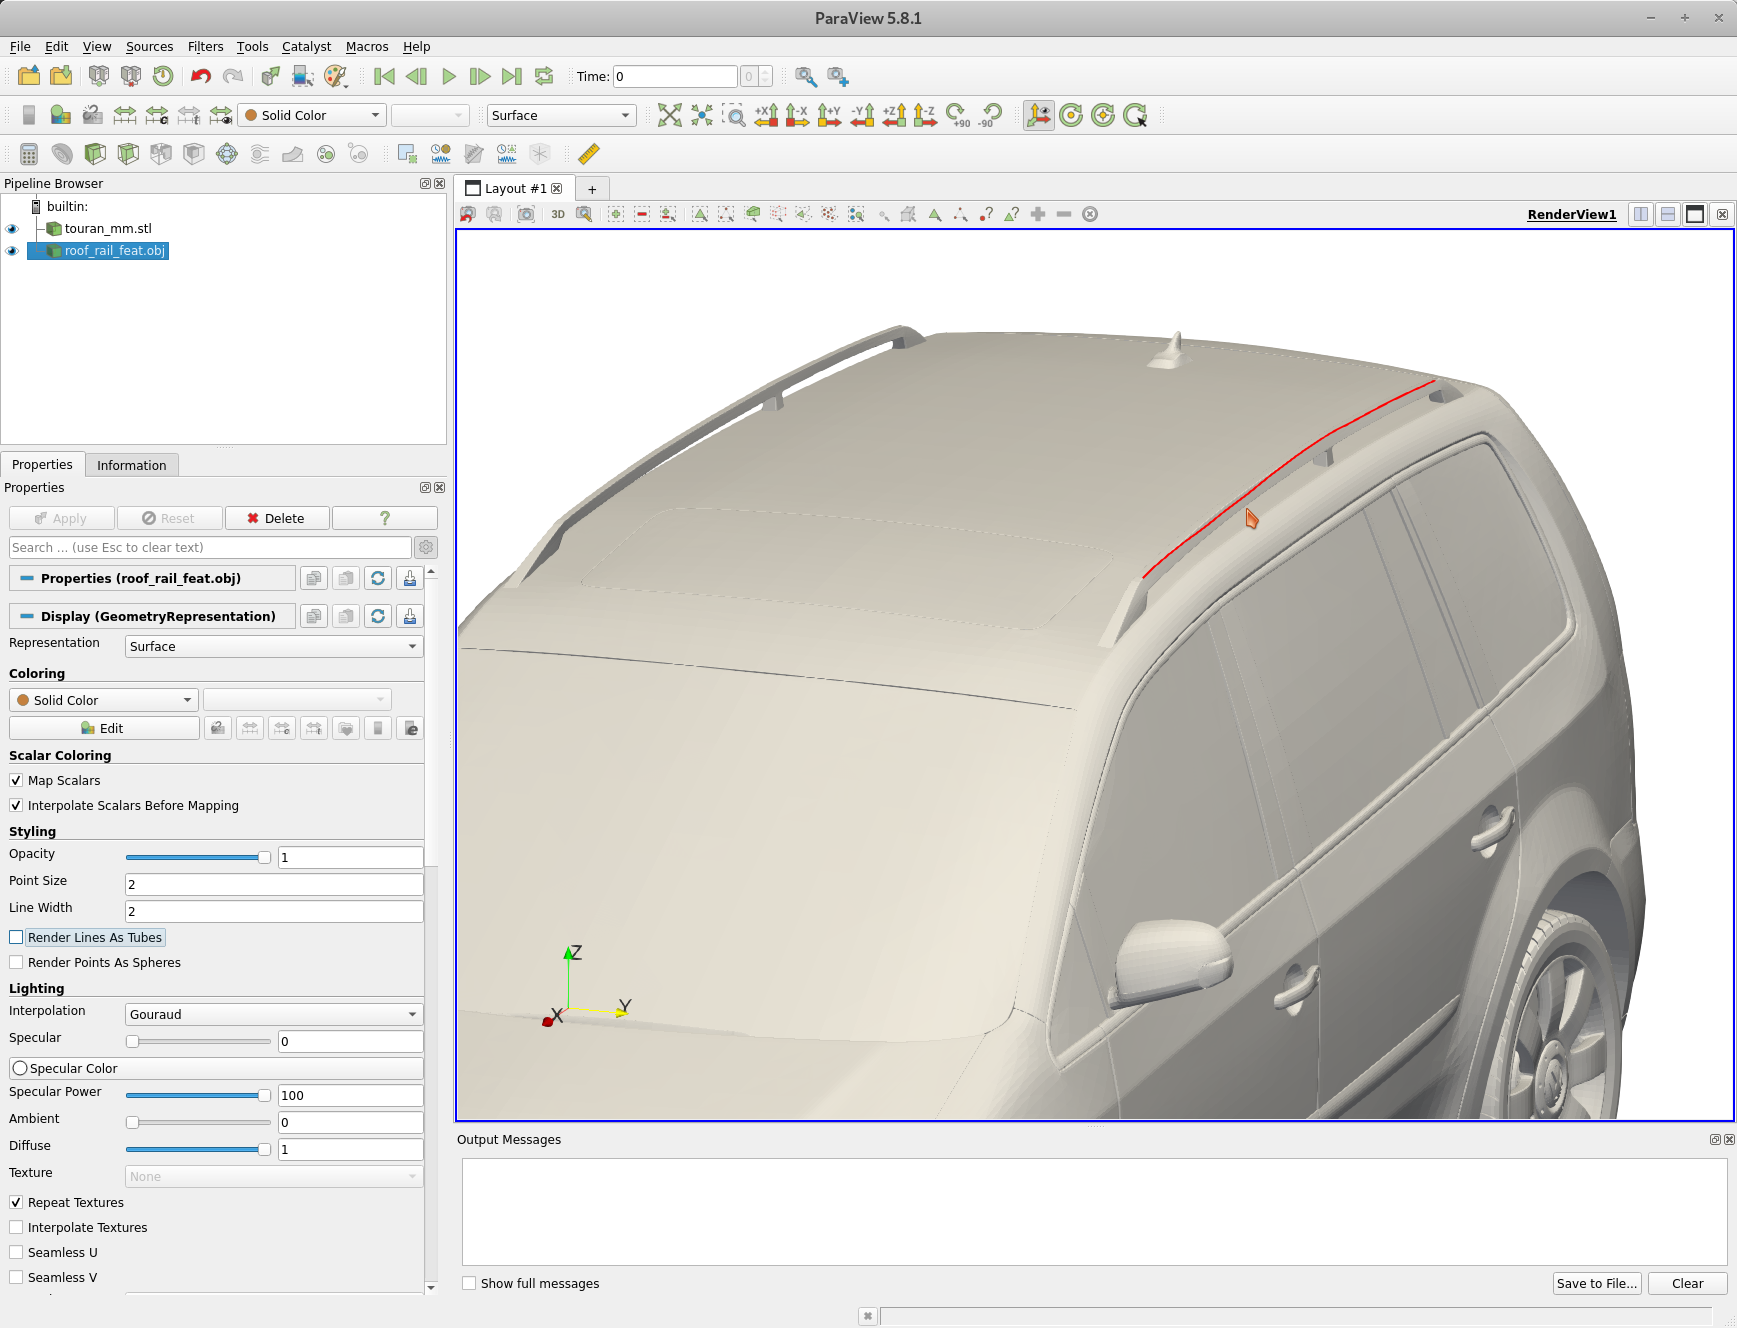
\includegraphics[width=0.75\linewidth]{figs/feature_edges_blender/12_view_paraview}

\item Finally, the OBJ files can be converted into OpenFOAM's eMesh format.
There is a tool called "surfaceFeatureConvert" in the OpenFOAM toolbox, which can perform this task.
The file type is recognized from the extension.
If not already done, the OpenFOAM environment needs to be loaded (here using the alias of1806):

\begin{lstlisting}
$ of1806
$ surfaceFeatureConvert roof_rail_feat.obj roof_rail_feat.eMesh
\end{lstlisting}


\end{enumerate}
